\documentclass[11pt]{article}
\usepackage[margin=1in]{geometry}
\usepackage{amsmath,amssymb,array,booktabs,graphicx}
\usepackage[T1]{fontenc}
\usepackage{lmodern}
\usepackage{microtype}
\usepackage[numbers,sort&compress]{natbib}
\usepackage{pgfplots}
\usepgfplotslibrary{groupplots}
\pgfplotsset{compat=1.18}
\usepackage[hidelinks]{hyperref}
\usepackage{url}
\newcommand{\bench}{GraphDecide}
\newcommand{\gap}{\operatorname{gap}}
\newcommand{\EPJevExact}{33/48}
\newcommand{\EPJevReturned}{48}
\newcommand{\EPJevCalls}{160}
\newcommand{\EPJevFailures}{0}
\newcommand{\EPJevExactFailures}{0}
\newcommand{\EPJevOptima}{2/16}
\newcommand{\EPGrammarExact}{30/48}
\newcommand{\EPGrammarReturned}{48}
\newcommand{\EPGrammarCalls}{160}
\newcommand{\EPGrammarFailures}{0}
\newcommand{\EPGrammarExactFailures}{0}
\newcommand{\EPGrammarOptima}{2/16}
\newcommand{\EPLargeThinkingExact}{47/48}
\newcommand{\EPLargeThinkingReturned}{47}
\newcommand{\EPLargeThinkingCalls}{66}
\newcommand{\EPLargeThinkingFailures}{17}
\newcommand{\EPLargeThinkingExactFailures}{1}
\newcommand{\EPLargeThinkingOptima}{0/16}
\newcommand{\EPSmallThinkingExact}{40/48}
\newcommand{\EPSmallThinkingReturned}{40}
\newcommand{\EPSmallThinkingCalls}{64}
\newcommand{\EPSmallThinkingFailures}{24}
\newcommand{\EPSmallThinkingExactFailures}{8}
\newcommand{\EPSmallThinkingOptima}{0/16}
\newcommand{\EPDeciderExact}{24/48}
\newcommand{\EPDeciderReturned}{48}
\newcommand{\EPDeciderCalls}{160}
\newcommand{\EPDeciderFailures}{0}
\newcommand{\EPDeciderExactFailures}{0}
\newcommand{\EPDeciderOptima}{0/16}
\newcommand{\EPKevExact}{23/48}
\newcommand{\EPKevReturned}{48}
\newcommand{\EPKevCalls}{160}
\newcommand{\EPKevFailures}{0}
\newcommand{\EPKevExactFailures}{0}
\newcommand{\EPKevOptima}{1/16}
\newcommand{\EPJevCommunityGap}{0.235880}
\newcommand{\EPKevCommunityGap}{0.113657}

\title{\bench: Benchmarking Decision Models on Graphs}
\author{Xianliang Yang\textsuperscript{1}\quad
Yapu Zhang\textsuperscript{2}\quad
Li Zhao\textsuperscript{1}\thanks{Corresponding author: \href{mailto:lizo@microsoft.com}{lizo@microsoft.com}.}\\[0.4em]
\small\textsuperscript{1}Microsoft\quad
\textsuperscript{2}Beijing University of Technology\\[0.3em]
\small\href{mailto:xianya@microsoft.com}{\texttt{xianya@microsoft.com}}\quad
\href{mailto:zhangyapu@bjut.edu.cn}{\texttt{zhangyapu@bjut.edu.cn}}\\
\small\href{mailto:lizo@microsoft.com}{\texttt{lizo@microsoft.com}}}
\hypersetup{
 pdftitle={GraphDecide: Benchmarking Decision Models on Graphs},
 pdfauthor={Xianliang Yang, Yapu Zhang, Li Zhao}
}
\date{September 27, 2026}
\begin{document}
\maketitle

\begin{abstract}
Can valid local decisions compose into good graph solutions? GraphDecide
evaluates Jev and open decision-oriented models on six exact graph tasks and
four irreversible construction tasks. Small graphs permit independently
checked labels, exact optima and own-history error analysis. Twelve
configurations share 960 instances: ten direct-decision configurations and
two GPT upper reference points with different reasoning budgets. Jev achieves
100\% adjacency accuracy but 61.43\% degree accuracy and 58.75\% distance
accuracy. Its mean TSP gap is 45.85 versus 100.90 for bounded Qwen3.5-27B;
on influence maximization their gaps are 0.600 and 0.425. Jev has smaller
construction gaps than added Qwen3.8-27B and Qwen2.5-72B configurations,
without establishing general parameter equivalence. A separate 952-instance
confirmation covers the original four configurations. Classical references,
presentation controls and probability audits distinguish valid actions from
correct decisions and competitive solutions. The benchmark characterizes
task-dependent capabilities, not a universal ranking or a fitted size limit.
\end{abstract}

\section{Introduction}
Decision-oriented models offer an alternative to open-ended generation:
rather than producing a free-form answer, they select an action from supplied
choices. Jev, developed by TypeSafe AI, is designed to return structured
choices and associated probabilities \cite{almeida2026jev}.
Open models also provide mechanisms for selecting among predefined options
\cite{semif2026,decider2026model,kev2026model,laya2026}.
These interfaces ease integration into deterministic programs, but restricting
outputs does not establish understanding of the underlying problem.
A model may recognize an edge without correctly counting a vertex's degree,
or repeatedly choose legal actions without constructing a good solution.
Beyond producing valid choices, to what extent can bounded decision models
support structural reasoning and sequential optimization?

Graphs provide a natural setting for this question. Local queries test
elementary discrimination; structural queries require reasoning beyond a
single edge; constructive tasks require decisions to remain useful as their
consequences accumulate. NLGraph and GraphArena establish graph reasoning
and solution verification as important evaluation directions
\cite{wang2023nlgraph,tang2025grapharena}.
Learned constructive optimization has a substantial history
\cite{khalil2017learning,kool2019attention}, and Jev-guided next-city
selection has already been explored in routing \cite{worldtour2026}.
Typed-decision evaluations such as JevBench assess bounded choices across
application domains \cite{jevbench2026}. These efforts motivate a
complementary diagnostic question: how does one-step correctness relate to
complete-solution quality when models follow their own previous decisions?

Answering this question requires more than final accuracy. Output validity,
mathematical correctness and optimization quality are distinct outcomes.
A legal trajectory may be far from optimal, while a method whose completed
solutions are all optimal may fail to finish many scheduled episodes.
Presentation, option order and decoding can also affect decisions without
changing the mathematical problem. Aggregate scores may therefore obscure
both accumulated errors and interface sensitivity. Evaluation should
separate these outcomes while retaining the trajectories and failures that
produced them.

We investigate three research questions:
\textbf{RQ1:} Which local and structural graph decisions distinguish Jev
from open trained decision models and bounded language-model baselines?
\textbf{RQ2:} Do useful one-step decisions compose into competitive solutions,
and where do actual trajectories irreversibly lose optimality?
\textbf{RQ3:} Which strengths and failures persist on new graphs and under
interface controls?
We introduce \emph{GraphDecide}, covering six single-step queries---adjacency,
degree, cycle detection, connectivity, distance thresholds and articulation
points---and four constructions: MaxCut, Manhattan traveling salesperson
(TSP), deterministic normalized linear-threshold influence maximization,
and modularity maximization with at most two communities.
At each step, a model receives the current public state and finite legal
actions. Deterministic code applies its choice without supplying oracle
actions, repairing incorrect responses or revising previous choices.
Small graphs permit independently checked answers, exact optimal objectives
and analysis of the best solution still reachable after each decision.

To reduce reliance on superficial statistics and repeated structures, we
match structural properties and pair opposite labels for selected binary
queries, and exclude graph structures overlapping a specified historical
pool. These controls do not establish immunity to all shortcuts or
pretraining contamination. Ten direct-decision configurations span Jev,
Decider, Kev, Laya and the Qwen family on 960 instances with 8--12 vertices;
GPT-5.4 and Astra provide reasoning references under different inference
settings (Section~\ref{sec:methods}). ``Jev-like'' denotes open
decision-oriented readouts, not verified reconstructions of Jev's
undisclosed architecture. We separately report query accuracy, mean objective
gap for complete legal solutions, and feasible coverage over all scheduled
episodes. Holding generation rules and sizes fixed, a new seed and
historical-topology exclusion yield 952 confirmation instances for Jev,
Qwen3.5-4B/9B grammar generation and Qwen3.5-4B candidate scoring,
not all twelve configurations. Four observations summarize the findings:
\begin{enumerate}
\item \textbf{Local discrimination does not imply structural reliability.}
Jev reaches 100\% adjacency accuracy, but 61.43\% degree and 58.75\%
distance accuracy. Open trained decision models do not recover its overall
exact-task profile (Table~\ref{tab:full-exact}).
\item \textbf{Sequential quality is task dependent.}
Jev has a smaller TSP gap than no-thinking, grammar-constrained Qwen3.5-27B;
the ordering reverses on deterministic influence maximization.
Classical and exact uniform-policy references show that outperforming a
neural configuration need not imply competitive optimization quality
(Section~\ref{sec:full-matrix}).
\item \textbf{Trajectory analysis identifies irreversible losses.}
The first TSP choice rules out every globally optimal completion in 3/40
Jev episodes, versus 22/40 for no-thinking, grammar-constrained Qwen3.5-4B.
Exact continuation values distinguish an early irreversible mistake from
a later choice that is optimal only within an already compromised state
(Appendix~\ref{sec:regret}).
\item \textbf{Selected failures recur, but rankings and choices can change.}
None of the four confirmation configurations reaches a MaxCut optimum,
as on the main set, while some taskwise orderings change
(Appendix~\ref{sec:confirmation}). Reversing option order flips all semantic
choices on twenty selected Qwen3.5-9B grammar articulation queries,
although accuracy remains 10/20 in both conditions
(Appendix~\ref{sec:controls}).
\end{enumerate}
Together, exact verification, trajectory analysis and controlled comparisons
make GraphDecide a diagnostic framework for individual graph decisions and
the solutions they collectively produce, not a universal model ranking.
Extended related work is in Appendix~\ref{sec:related-work}.
Code and aggregate results are released at
\url{https://github.com/microsoft/HeurAgenix.git},
on branch \texttt{graph\_benchmark}, in
\texttt{benchmarks/graphdecide}. Raw provider logs and model weights are
not included in this code release.

\section{Tasks and benchmark data}
\label{sec:tasks}
Public inputs contain graph structure and the current question, never
generation-family labels, reference answers or optimum values.
Unless specified otherwise, graphs are simple, undirected and unweighted,
with integer vertices including isolates.

\begin{table}[ht]
\centering\small
\begin{tabular}{llrr}
\toprule
Task & Answer or objective & Cases & Choices/case\\
\midrule
Adjacency & Shared edge: yes/no & 80 & 1\\
Degree & Neighbor count: $0,\ldots,n-1$ & 400 & 1\\
Cycle & Cycle exists: yes/no & 80 & 1\\
Connectivity & Path exists: yes/no & 80 & 1\\
Distance & Distance $\leq h$: yes/no & 80 & 1\\
Articulation & Components increase: yes/no & 80 & 1\\
\midrule
MaxCut & Maximize crossing edges & 40 & $n-1$\\
Manhattan TSP & Minimize closed-tour length & 40 & $n-2$\\
Deterministic LT & Maximize activated nodes & 40 & 2\\
Modularity & Maximize two-group modularity & 40 & $n-1$\\
\bottomrule
\end{tabular}
\caption{Canonical task inventory on the shared $n=8,\ldots,12$ bank.
Counts are scheduled cases per configuration, not independent graphs.
Construction choices form one complete own-history trajectory.}
\label{tab:task-overview}
\end{table}

\paragraph{Exact decisions.}
The six tasks ask whether two vertices share an edge (\emph{adjacency}),
the number of distinct neighbors (\emph{degree}), whether any component has
a simple cycle of length at least three (\emph{cycle}), whether a path
connects a pair (\emph{connectivity}), whether shortest-path distance is at
most a supplied threshold (\emph{distance}), and whether deleting a vertex
increases the total component count (\emph{articulation}). Degree offers
all $n$ answers from 0 to $n-1$; the other tasks are binary. Distance
challenge pairs have finite distances exactly $h$ and $h+1$.

\paragraph{Irreversible constructions.}
MaxCut assigns vertices in order to two sides, fixing vertex 0 in A,
to maximize crossing edges in $n-1$ choices. Manhattan TSP starts at city 0
and chooses unvisited cities in $n-2$ decisions; the final city and return
edge are forced, and full closed-tour distance is minimized.
Deterministic normalized linear-threshold (LT) influence selects two
distinct seeds on a directed graph to maximize final activated nodes.
Incoming weights are $1/d^-(v)$, threshold is $1/2$, seeds activate
simultaneously, and diffusion is synchronous and irreversible.
The modularity task assigns vertices to at most two communities, again
fixing vertex 0, to maximize standard resolution-1 modularity
\cite{newman2004community}. Empty sides and one community are legal.
This is neither unrestricted community detection nor the random-threshold
LT model: its classical submodularity guarantee is not assumed
\cite{kempe2015influence}. Exact contracts and invariants are in
Appendices~\ref{app:task-details} and \ref{app:contracts}.

\paragraph{Consecutive sizes and coverage.}
Development contains 356 realized cases at every integer size 5--12;
the canonical challenge contains 960 at sizes 8--12. At each challenge
size there are sixteen queries for each binary task, $8n$ degree queries,
and eight episodes for each construction. Thus every model receives
800 exact queries and 160 constructions, requiring at most 1,920 calls.
Four development cases were not generated within the bounded proposal
budget; the canonical challenge has no omissions.
The separate prospective confirmation realizes 952 of 960 requested
cases, retaining eight missing cycle cases as generation shortfalls.
Full counts and chronology are in Appendix~\ref{app:data-details}.

\paragraph{Controls and exact verification.}
Heterogeneous graph-generation procedures vary structure within sizes.
Binary positive/negative pairs match audited degree-based attributes:
query tasks generally share a graph; cycle twins share $n,m$ and the degree
multiset. The audited cells are label-balanced, giving a 50\% empirical
lookup ceiling for those attributes, not immunity to every shortcut.
Graph fingerprints select candidate identity matches; exact isomorphism
checks enforce exclusion against the recorded prior pool. TSP identity uses
weighted distance graphs and LT uses directed topology.

Labels and objectives are independently checked. Adjacency, distance and
articulation oracles were tested on all 1,024 labeled five-vertex graphs;
subset dynamic programming checks TSP optima, while small partition and seed
spaces permit exhaustive checks. Public request construction is separate
from privileged references. ``Independent'' here means separate computation
within this project, not external replication. The canonical bank was
already inspected before later model extensions; it is not a newly blind
test. Locally frozen registrations are not external preregistration.

\section{Evaluation protocol}
\label{sec:methods}
\paragraph{Models and budgets.}
The ten direct-decision configurations are Jev's native action selection;
no-thinking Qwen3.5-4B/9B/27B grammar generation \cite{qwen2026qwen35}; a Qwen3.5-4B
candidate-token-score reference; trained Decider-2B v11, Kev-4B and Laya;
and full-BF16 Qwen3.8-27B \cite{qwen2026qwen38} and
Qwen2.5-72B-Instruct \cite{qwen2024qwen25}.
Grammar configurations use greedy legal-choice generation with a 64-token
ceiling. The larger/newer local lanes use a 180-second request deadline;
thinking is disabled for Qwen3.8, while Qwen2.5 uses its standard instruct
template without added reasoning. The older-generation 72B is not a scale-only
ablation of Qwen3.5/3.8. GPT-5.4 and Astra use tool-free default reasoning,
a 4,096-token ceiling and a 180-second deadline, and remain separately grouped.
No Jev outputs are used to train a replacement. Checkpoints, serving settings
and compatibility qualifications are in Appendix~\ref{app:method-details}.

\paragraph{Interactions and failures.}
Every model receives the same initial logical request with explicit action
descriptions. Each later state follows that model's actual previous choices,
not teacher-forced or oracle prefixes. A valid native Jev action is not
replaced by probability argmax; probability conformance is audited separately.
Unsupported inputs, timeouts and invalid outputs remain in scheduled
denominators. There is no answer repair, silent truncation or replacement
of failed cases. Feasibility means a valid answer or complete legal trajectory,
not mathematical correctness. All tied optima are accepted.

\paragraph{Metrics and uncertainty.}
Exact-task accuracy is the equal-weight mean of five size-specific
accuracies. Degree's pooled correct count is different because each size has
$8n$ queries. The primary construction-quality metric is mean additive
objective gap over feasible completed episodes, always accompanied by
feasible coverage over all scheduled episodes:
\[
\gap_i=
\begin{cases}
f_i^\star-f_i,&\text{maximization},\\
f_i-f_i^\star,&\text{minimization}.
\end{cases}
\]
We average per-episode gaps, not optimum-hit indicators. Units are crossing
edges, Manhattan distance, activated nodes and modularity; absolute gaps
must not be pooled across tasks or interpreted as percentages.
Zero conditional gap does not imply zero failures. Optimum-hit counts
are supplementary (Appendix~\ref{app:construction-hits}).

The twelve-configuration tables are descriptive point estimates, not
family-wise significance claims. Original four-configuration uncertainty
uses 2,000 size-stratified paired bootstrap replicates over clusters joining
graph identity and matched-pair relations, rather than treating related
queries as independent (Appendix~\ref{app:method-details}).
Generation omissions have no model prediction and are not scored as model
errors; model failures on generated cases remain in the denominator.
Only the original four configurations receive prospective new-graph
confirmation; model extensions do not inherit that replication.

\section{Canonical results}
\label{sec:full-matrix}
The complete comparison comprises 11,520 scheduled episode evaluations on
the same 960 instances, not 11,520 independent graphs. Frozen results are
reused when adding models. The public presentation contains
720 task/size/configuration cells. Historical pilots and legacy Astra
protocols are separate, not mixed into the main columns.

\begin{table}[t]
\centering\small
\resizebox{\textwidth}{!}{\begin{tabular}{lrrrrr}
\toprule
Model & Exact feasible & Construct feasible & Input rejects & Exec. failures & Unattempted \\
\midrule
Jev & 800/800 & 160/160 & 0 & 0 & 0 \\
Qwen4 G & 800/800 & 160/160 & 0 & 0 & 0 \\
Qwen9 G & 800/800 & 160/160 & 0 & 0 & 0 \\
Qwen27 G & 800/800 & 160/160 & 0 & 0 & 0 \\
Qwen3.8-27B & 800/800 & 160/160 & 0 & 0 & 0 \\
Qwen2.5-72B & 800/800 & 160/160 & 0 & 0 & 0 \\
Qwen4 scores & 800/800 & 160/160 & 0 & 0 & 0 \\
Decider & 800/800 & 160/160 & 0 & 0 & 0 \\
Kev & 800/800 & 160/160 & 0 & 0 & 0 \\
Laya & 800/800 & 151/160 & 9 & 0 & 0 \\
\midrule
GPT-5.4 & 800/800 & 151/160 & 0 & 9 & 0 \\
Astra & 800/800 & 160/160 & 0 & 0 & 0 \\
\bottomrule
\end{tabular}
}
\caption{Full canonical coverage. Exact feasibility means a valid returned
answer, not a correct answer. Construction feasibility requires a complete
legal trajectory. Input rejects and execution failures are episode counts.
All twelve configurations retain 960 scheduled cases. The lower block contains
GPT default-reasoning anchors, not matched-compute direct-decision baselines.}
\label{tab:full-coverage}
\end{table}

\paragraph{Coverage.}
All configurations except Laya and GPT-5.4 complete 960/960 episodes.
Laya rejects nine LT inputs at its lossless context/head limits, leaving
31/40 feasible LT episodes. GPT-5.4 retains nine construction timeouts:
36/40 cut, 39/40 TSP, 40/40 LT and 36/40 modularity episodes are feasible.
Every other construction cell has 40/40 feasible episodes.
Table~\ref{tab:full-coverage} gives the complete counts; integrity checks
are in Appendix~\ref{app:coverage-integrity}.

\begin{table}[t]
\centering\small
\resizebox{\textwidth}{!}{\begin{tabular}{lrrrrrr}
\toprule
Model & Adjacency & Degree & Cycle & Connectivity & Distance & Articulation \\
\midrule
Jev & 100.00 & 61.43 & 66.25 & 85.00 & 58.75 & 65.00 \\
Qwen4 G & 60.00 & 18.32 & 55.00 & 50.00 & 50.00 & 50.00 \\
Qwen9 G & 58.75 & 26.99 & 51.25 & 53.75 & 42.50 & 50.00 \\
Qwen27 G & 98.75 & 47.70 & 63.75 & 80.00 & 52.50 & 47.50 \\
Qwen3.8-27B & 90.00 & 45.50 & 61.25 & 85.00 & 48.75 & 50.00 \\
Qwen2.5-72B & 92.50 & 41.24 & 50.00 & 86.25 & 60.00 & 46.25 \\
Qwen4 scores & 77.50 & 23.89 & 51.25 & 51.25 & 52.50 & 50.00 \\
Decider & 58.75 & 12.09 & 50.00 & 50.00 & 46.25 & 50.00 \\
Kev & 78.75 & 19.88 & 57.50 & 58.75 & 51.25 & 45.00 \\
Laya & 50.00 & 10.87 & 50.00 & 50.00 & 50.00 & 50.00 \\
\midrule
GPT-5.4 & 100.00 & 100.00 & 100.00 & 100.00 & 100.00 & 100.00 \\
Astra & 100.00 & 100.00 & 100.00 & 100.00 & 100.00 & 100.00 \\
\bottomrule
\end{tabular}
}
\caption{Canonical exact-task macro-size accuracy (\%). Qwen4/9/27 G denote
Qwen3.5 no-thinking grammar configurations; other Qwen generations are named.
GPT default-reasoning anchors form a separate lower block.}
\label{tab:full-exact}
\end{table}

\paragraph{RQ1: Strengths are task dependent.}
Jev's 100\% adjacency accuracy does not extend to uniform structural
reliability: degree is 61.43\%, cycle 66.25\%, and distance 58.75\%
(Table~\ref{tab:full-exact}). Open trained readouts do not recover its
exact-task profile. Kev reaches 78.75\% adjacency and 19.88\% degree;
Decider reaches 58.75\% and 12.09\%. Laya selects \texttt{yes} on all
400 binary queries. Native-score, mapping and replay checks retain that
outcome as observed behavior, not an assumed parser failure.

Jev's exact-task point estimates exceed bounded Qwen3.5-27B on all six
tasks, but this does not establish general parameter equivalence.
The newer Qwen3.8-27B and larger Qwen2.5-72B reach degree macro accuracies
of 45.50\% and 41.24\%, respectively, not their pooled rates of 44.50\%
and 40.50\%. The 72B connectivity and distance estimates exceed Jev by
only one answer out of eighty each. Model size and generation therefore
do not induce a monotone ordering under this bounded protocol.

\begin{table}[t]
\centering\small
\begin{tabular}{lrrrr}
\toprule
Model & MaxCut & TSP & Deterministic LT & Modularity \\
\midrule
Jev & 8.1500 & 45.8500 & 0.6000 & 0.1694 \\
Qwen4 G & 11.1250 & 338.1500 & 2.6250 & 0.2900 \\
Qwen9 G & 11.0500 & 306.4500 & 3.7250 & 0.3203 \\
Qwen27 G & 8.0250 & 100.9000 & 0.4250 & 0.2810 \\
Qwen3.8-27B & 11.1500 & 183.7000 & 2.6750 & 0.3012 \\
Qwen2.5-72B & 9.7750 & 152.4000 & 1.9500 & 0.2645 \\
Qwen4 scores & 9.2000 & 351.0000 & 4.1250 & 0.2810 \\
Decider & 11.1250 & 355.7000 & 4.1000 & 0.2810 \\
Kev & 11.0750 & 349.6500 & 0.6000 & 0.2502 \\
Laya & 15.2500 & 344.7500 & 2.8710 & 0.3039 \\
\midrule
GPT-5.4 & 0.0000 & 0.0000 & 0.0000 & 0.0000 \\
Astra & 0.0000 & 0.0000 & 0.0000 & 0.0000 \\
\bottomrule
\end{tabular}

\caption{Primary construction outcome: mean additive objective gap over
feasible completions; lower is better. Units differ across columns.
All cells use forty episodes except Laya LT (31), GPT-5.4 cut (36),
TSP (39) and modularity (36). Different coverage is not a matched-subset
comparison.}
\label{tab:full-gaps}
\end{table}

\paragraph{RQ2: Quality is not optimum-hit frequency.}
Jev's TSP gap is 45.85, compared with 100.90 for Qwen3.5-27B and
349.65 for Kev (Table~\ref{tab:full-gaps}). LT reverses the Jev--Qwen3.5-27B
ordering: their gaps are 0.600 and 0.425. Kev ties Jev at 0.600;
its larger optimum-hit count does not establish better mean quality.
Qwen3.5-27B also has a slightly smaller cut gap (8.025 versus 8.150),
whereas Jev has the smaller modularity gap (0.1694 versus 0.2810).
These are taskwise observations, not established significant differences.

Jev has smaller mean gaps on all four constructions than either added
Qwen3.8-27B or Qwen2.5-72B configuration, each with complete feasible
coverage. In TSP their gaps are 183.70 and 152.40, respectively.
This supports a direct-decision advantage on these instances, not a
claim that Jev matches a general 72B model. No equal-hardware latency comparison
or causal architecture attribution follows from these scores.

Absolute quality requires algorithmic references. Jev's MaxCut gap of
8.150 exceeds the uniform legal policy's exact expected gap of 5.325;
classical cut search achieves 0.450. Nearest-neighbor plus 2-opt has
TSP gap 0.200 versus Jev's 45.850. These algorithms may revise choices
and are quality references, not equal-budget online competitors.
Relative neural superiority is not competitiveness with classical solvers.
Own-history continuation analysis gives a complementary error measure:
over 640 constructions of the original four configurations, stepwise
continuation losses telescope to final gap for all 4,480 decisions.
Jev loses TSP optimality at its first choice in 3/40 episodes, compared
with 22/40 for grammar-4B (Appendix~\ref{sec:regret}).

\paragraph{Reasoning anchors.}
Both GPT configurations answer all 800 exact queries correctly.
Astra reaches zero gap with all 160 constructions feasible; GPT-5.4
reaches zero conditional gap with 151/160 feasible. This demonstrates
that stronger reasoning can solve these small instances, without making
matched-compute claims or requiring further difficulty escalation.

\section{Robustness and interpretation}
\label{sec:discussion}
\paragraph{RQ3: Confirmation has a defined scope.}
The topology-excluded prospective confirmation contains 952 new instances
for the original four configurations, not all twelve.
Jev retains perfect adjacency, and all four again have larger MaxCut gaps
than the uniform policy. Some rankings change, so confirmation supports
selected patterns rather than every canonical estimate
(Appendix~\ref{sec:confirmation}).
Likewise, Kev's community advantage in an exploratory 64-case panel does
not persist on the canonical bank. The smaller and larger panels are
different graph sets, not a paired sample-size intervention.

\paragraph{Interface and probability controls.}
Option/state transformations expose semantic-choice reversals that
aggregate accuracy can hide. At an identical token prefix, 4B
candidate-score argmax and masked greedy agree on 100/100 states:
argmax alone does not explain the main pipeline's gains.
A separate CPU/GPU SemIf check matches choices but exceeds the registered
0.01 probability-error tolerance; the failed numerical reproduction
gate remains unresolved. Hence the score baseline is an interface
reference, not a certified reproduction.
Laya's option-reversal pilot argues against a simple first-option bias,
not against all prompting effects.

Numeric probability output does not imply calibration
\cite{gneiting2007proper,guo2017calibration}. Jev's above-chance distance
accuracy coexists with probability losses worse than uniform on
common-valid audit rows. These diagnostics separate mathematical
correctness, action validity and probability quality; they do not prove
absence of every implementation error. Full controls and probability
tables remain in Appendix~\ref{sec:controls}.

\paragraph{Size and speed are bounded observations.}
Consecutive sizes reveal different profiles, not a fitted common boundary.
Jev degree accuracy decreases from 70.3\% at $n=8$ to 49.0\% at $n=12$;
cycle decreases from 81.25\% to 50\%, with nonmonotone intermediate cells.
Adjacency stays perfect. Binary cells have only sixteen queries and
construction cells eight episodes, and degree's number of classes grows.
These observations do not identify ``failure at twelve vertices.''
In the original four-configuration timing panel, Jev's median response is
70.01 ms, versus 64.41 ms for 4B candidate scoring and 94.24 ms for
4B grammar generation. Jev is not invariably fastest; different hardware,
network paths and serving conditions prevent architecture or cost attribution
(Appendix~\ref{app:original-results}).

\section{Limitations and conclusion}
\label{sec:limits}
Small graphs enable exact checking but do not establish operational-scale
performance, size-OOD generalization or an ordering of causal difficulty.
Finite generation procedures, degree conditioning and matching determine
the tested distribution. Prior-topology exclusion is local, not proof
against pretraining contamination. Later model choices use inspected banks;
only four configurations have prospective new-graph confirmation.
Taskwise estimates and exploratory bootstrap intervals do not correct
all selection or multiplicity. Jev is closed, renderings and budgets are
not fully matched, and trained readouts use compatible rather than
identical upstream environments. Extended limitations and protocol
details are retained in the appendices.

The artifacts contain synthetic graph states, not personal-network data;
deterministic LT is not a validated model of human behavior. Public
aggregates and scoring artifacts exclude credentials and raw provider
responses. Local registrations and independent replay are not third-party
attestation; extension-artifact distribution and publication permissions
remain release requirements.

GraphDecide shows why valid choices, exact reasoning and good complete
solutions must be evaluated separately. Jev has task-specific advantages
over open readouts and several bounded Qwen configurations, including
the added 72B baseline, yet remains far from classical optimization
quality. Mean gaps reveal differences hidden by optimum-hit counts.
The supported result is a capability profile with explicit uncertainty,
not a universal model ranking. Fresh-graph confirmation and controlled
transition-region studies are more informative next steps than increasing
size solely because the GPT anchors remain successful.
\label{sec:main-end}

\clearpage
\bibliographystyle{plainnat}
{\raggedright\bibliography{references,expanded-references}}

\clearpage
\appendix
\section{Task and interaction contracts}
\label{app:task-details}
Unless stated otherwise, $G=(V,E)$ is simple, undirected and unweighted, with
integer vertices $V=\{0,\ldots,n-1\}$, including isolates. Public data contain
the graph and the query; action identifiers are strings. Generation families,
reference answers, optimum values, and paired-label annotations are not model
inputs.

\subsection{Six exact decisions}
\begin{description}
 \item[Adjacency.] Decide whether $\{u,v\}\in E$ for distinct supplied vertices.
 \item[Degree.] Return $d(v)$ from the full choice set $\{0,\ldots,n-1\}$.
 The growing output cardinality is an explicit size confound.
 \item[Cycle.] Decide whether any component contains an undirected simple
 cycle of length at least three.
 \item[Connectivity.] Decide whether a path connects the supplied vertices.
 \item[Distance.] Decide whether the shortest-path distance is at most a
 supplied threshold $h$. Matched challenge pairs have finite distances
 exactly $h$ and $h+1$, rather than disconnected negative examples.
 \item[Articulation.] Decide whether deleting a supplied vertex increases
 the total number of connected components, including on disconnected graphs.
\end{description}

\subsection{Four irreversible constructions}
\paragraph{MaxCut.}
Vertex 0 is fixed in side A. In increasing vertex order, the model assigns
each remaining vertex to A or B, using $n-1$ decisions. The maximized objective
is the number of edges crossing the partition. Empty sides are legal.

\paragraph{Manhattan TSP.}
Distinct integer coordinates define a complete weighted graph with
$d_{ij}=|x_i-x_j|+|y_i-y_j|$. Starting at 0, the model selects the next unvisited
vertex for $n-2$ decisions. The final unvisited vertex and edge returning to 0
are then forced. This deterministic completion is part of the contract,
not answer repair. The minimized objective is full tour length.

\paragraph{Deterministic normalized linear threshold (LT).}
On a directed graph, every incoming edge to $v$ has weight
$1/d^-(v)$ and the threshold is $1/2$, with equality activating.
The model selects two distinct seeds, which activate simultaneously at time
zero. Subsequent updates are synchronous and irreversible. A zero-indegree
nonseed never activates. The maximized objective is final active-set size.
This fixed-threshold variant is not the random-threshold classical LT model;
we do not import its submodularity or greedy approximation guarantee.

\paragraph{At-most-two-community modularity.}
Using the same fixed-0, $n-1$ binary assignment protocol, maximize
\[
 Q(c)=\frac{1}{2m}\sum_{u,v}
 \left(A_{uv}-\frac{d_ud_v}{2m}\right)\mathbf{1}[c_u=c_v].
\]
All-A is a valid one-community solution with $Q=0$.
This is a restricted bipartition task, not unrestricted community detection.

\paragraph{Shared policy.}
Every tied optimum is accepted; matching a particular reference trajectory
is unnecessary. Models see their own previous choices, not teacher-forced
prefixes, except in explicitly separate diagnostic controls. Invalid or
incomplete episodes remain infeasible, with no imputed objective, retries,
or silent substitution of an action.

\section{Controlled data generation and verification}
\label{app:data-details}
\begin{table}[t]
\centering\small
\begin{tabular}{lrrr}
\toprule
Task & Development & Challenge & Decisions per instance\\
\midrule
Adjacency & 32 & 80 & 1\\
Degree & 136 & 400 & 1\\
Cycle & 30 & 80 & 1\\
Connectivity & 32 & 80 & 1\\
Distance & 32 & 80 & 1\\
Articulation & 30 & 80 & 1\\
MaxCut & 16 & 40 & $n-1$\\
TSP & 16 & 40 & $n-2$\\
Deterministic LT & 16 & 40 & 2\\
Modularity & 16 & 40 & $n-1$\\
\midrule
Total & 356 & 960 & 668 / 1,920 per model\\
\bottomrule
\end{tabular}
\caption{Dataset counts and maximum calls. An additional forty weighted TSP
instances support wording confirmation and bring the release to 1,356.
They are not additional rows of the canonical comparison.}
\label{tab:data}
\end{table}

\subsection{Size, structure and pairing}
Development covers each integer $n=5,\ldots,12$ with two repetitions; the
structural challenge covers $n=8,\ldots,12$ with eight repetitions.
Each size/repetition requests $n+14$ instances and $4n+8$ maximum calls.
Size is a consecutive descriptive axis, not a guarantee of increasing
difficulty or a causal intervention holding every other property fixed.

We use heterogeneous block, core--periphery and geometric procedures for
query tasks; forests and degree-preserving switches for cycle twins;
small-world and switched regular bases for cuts; clustered or perturbed-ring
coordinates for TSP; layered directed acyclic graphs for LT; and heterogeneous
blocks for modularity. These are finite, overlapping procedures, not uniform
samples from all graphs or disjoint mathematical families. Degree conditioning
can change a proposal's original family characteristics.

For adjacency, connectivity and distance, positive and negative queries
share a graph and have identical unordered endpoint-degree signatures.
Articulation queries share a graph and equal vertex degrees. Cycle twins
are different graphs with equal $n$, $m$ and degree multiset but opposite
labels. All five binary tasks are balanced within the audited cells defined by
$n$, $m$, degree multiset, query degrees and (where applicable) $h$, giving a 50\% empirical
lookup ceiling for those cells. This does not rule out unexamined shortcuts.
For example, component count plus $n,m$ determines undirected cycle existence.

Generation allows at most 128 proposals per cell and records unsupported
cells rather than weakening constraints. Four development instances are
missing: one cycle pair and one articulation pair at $n=5$.
Exhaustion of all 34 unlabeled five-vertex graphs finds one eligible
forest/cyclic topology pair but two eligible articulation topologies; the
latter shortfall is therefore a generator-support/budget limitation, not
a theorem of impossibility. The original 960-instance challenge has no omissions.

\subsection{Identity exclusion and evidence chronology}
The original challenge excludes an audited pool of 1,040 exact-labeled
deduplicated records from 121 earlier artifacts. Fingerprints select candidate
buckets; exact VF2 comparisons determine identity. TSP uses complete weighted
distance graphs, and LT uses directed topology. Independent checks found no
prior overlap and no same-task duplicate across nominally independent
clusters. The 1,040 records are not claimed to be 1,040 isomorphism classes.

Crucially, the common-interface matrix in this paper reuses these already
inspected banks. Its protocol was frozen before its own calls, but it is
\emph{not a newly blind test}. Earlier development diagnosed wording and
conformance issues. A subsequent prospective confirmation excludes these
banks and retains its own results, including missing cells, rather than replacing
them after inspecting outcomes (Section~\ref{sec:confirmation}).
We preserve the chronological distinction
between original strict experiments, diagnostic controls and the revised
common-interface matrix.

\paragraph{Meaning of registration and independent checking.}
Here, ``registered'' or ``preregistered'' means a locally persisted design
record frozen before the specified calls (and, for the confirmation, before
generation), not a deposit in an external public preregistration registry.
Source and artifact hashes detect changes relative to those records; they
are not third-party timestamps or cryptographic proof of the full chronology.
Independent verification means separate replay or mathematical computation
within this project, not replication by an external research group.

\subsection{Independent truth and artifact boundaries}
New adjacency, distance and articulation oracles were exhaustively checked
on all 1,024 labeled five-vertex graphs. Every released label, feasible
reference, baseline and optimum passes independent validation; TSP uses exact
subset dynamic programming and an independent optimum check, while the small
partition and seed spaces permit exhaustive verification.

The portable artifact separates five public fields (identifier, task, kind,
state, query budget), private references, and analysis metadata. Its request
builder does not read references. Offline scoring is deliberately privileged:
giving that scorer to a model would change the benchmark. The archive was
extracted into an isolated Python process and all 1,356 instances were
verified without importing model clients, Torch or the Copilot SDK.

\section{Evaluation design}
\label{app:method-details}
\subsection{Evidence sets and permissible comparisons}
Table~\ref{tab:evidence-map} distinguishes the complete canonical comparison
from its four-configuration diagnostic and confirmation subsets.
Reusing graph instances allows paired comparisons
but does not add independent test graphs. Freezing a later model's protocol
before its calls does not make an already inspected bank a blind holdout.

\begin{table}[t]
\centering\small
\begin{tabular}{>{\raggedright\arraybackslash}p{0.22\textwidth}r>{\raggedright\arraybackslash}p{0.52\textwidth}}
\toprule
Evidence set & Cases per method & Interpretation\\
\midrule
Original four-configuration matrix & 1,316 & 356 development and 960
inspected challenge cases.\\
Prospective confirmation & 952 & Same four configurations; new seed and
prior-topology exclusion, but unchanged generator procedures and sizes.\\
Canonical GPT-5.4 & 960 & Reuses the inspected challenge; identical initial
logical requests, not matched reasoning or compute.\\
Full cross-family matrix & 960 & Twelve configurations on that same challenge,
including canonical Astra; ten direct-decision configurations and two
separately labeled GPT reasoning anchors.\\
Larger/newer local extension & 960 & Qwen3.8-27B and Qwen2.5-72B-Instruct,
included in the twelve above; not additional graphs or a scale-only ablation.\\
Legacy Astra & 960 & Same challenge graphs, different instructions and
option descriptions; separate protocol.\\
Expanded local/readout panel & 64 & Reuses selected confirmation cases at
$n=8,12$; exploratory, not a new blind replication.\\
\bottomrule
\end{tabular}
\caption{Core evidence sets, not a sum of independent graphs. Later
presentation, probability and deadline controls reuse their explicitly
named banks. Cases are scheduled episodes, not necessarily completed ones.}
\label{tab:evidence-map}
\end{table}

\subsection{Completed common-interface configurations}
Every method receives the same initial logical request, including explicit
action descriptions. Questions specify mathematics rather than requiring a
wire encoding that could conflict with a letter-based readout. TSP explicitly
names the current endpoint and actual visited prefix.

\begin{description}
 \item[Jev action.] Native supplied choices under an explicitly registered
 action-eligibility policy. Expected model, response shape, legal choice,
 probability keys and finite ranges, confidence and usage must still validate.
 Probability normalization and choice/argmax disagreement are separately
 recorded observations, not reasons to replace the supplied action.
 \item[4B and 9B grammar.] Qwen3.5-4B and Qwen3.5-9B, greedy no-thinking
 generation, 64-token ceiling and legal-choice grammar, with the existing
 output parser. Thinking-enabled extensions are reported separately.
 \item[4B scores.] The existing 4B checkpoint with pinned SemIf-style
 rendering and exact requested candidate-token log probabilities from vLLM.
 The chosen action is the conditional argmax over \emph{all} candidates, not
 a natural top-$K$ approximation. One API-generated token is unused for
 selection and is counted in resource accounting.
 \item[27B grammar.] Qwen3.5-27B with the same no-thinking, 64-token,
 legal-choice grammar policy and a 180-second request deadline.
 \item[Larger/newer local grammar.] Qwen3.8-27B and Qwen2.5-72B-Instruct
 use full BF16 weights, greedy legal-choice grammar, a 64-token ceiling
 and a 180-second deadline. Thinking is explicitly disabled for Qwen3.8;
 Qwen2.5 uses its standard instruct template without added reasoning.
 They use two and four RTX A6000 GPUs, respectively. The 72B checkpoint
 is an older-generation dense model, not a scale-only variant of Qwen3.5/3.8.
 \item[Trained Jev-like readouts.] Decider-2B v11 and Kev-4B use their
 pinned upstream native inference paths; Laya uses its encoder and trained
 choice head in CPU FP32. Lossless context checks remain binding.
 These are compatible-runtime evaluations, not certifications of identical
 upstream environments.
 \item[Reasoning anchors.] GPT-5.4 and Astra use tool-free, default-reasoning
 clients with 4,096 output tokens and a 180-second deadline. They are
 separated from the ten direct-decision configurations throughout.
\end{description}
No Jev outputs are used to train or distill a replacement model.
The original four-configuration matrix retained the existing RTX A6000
services. Later GPU extensions used recorded resource leases and restored
the original services. The earlier extensions protected 4B/9B;
the final BF16 extension temporarily leased all four GPUs with authorization
and restored all original endpoints after completion.
The 4B generation/scoring methods share a physical-resource lock.
The checkpoint, renderer, environment and per-call settings are recorded.
This controls some factors, but the 4B readout comparison also changes rendering
and cannot identify a pure causal effect of the scoring rule.

\paragraph{A failed reproduction check is retained.}
On twelve matched CPU SemIf probes, both GPU scoring routes matched every
chosen action. However, maximum probability errors were 0.0166305 for requested
token scores and 0.0379656 for teacher forcing, both exceeding the pre-frozen
0.01 threshold; the routes differed by 0.0213351. Independent token indexing
and high-precision softmax recomputation found no parser mismatch. The
numerical cause remains unresolved. Thus ``4B scores'' is an independent
reference using SemIf rendering, not certified numerical reproduction of
CPU SemIf, and the failed gate is not relaxed.

\subsection{Metrics and statistical units}
For an exact task, the primary accuracy is the mean of the size-specific
accuracies, with invalid/unattempted scheduled cases retained in denominators.
For degree, macro-size and pooled accuracy differ because there are $n$
classes per size. The primary construction-quality metric is mean additive
objective gap over feasible completed episodes, accompanied by feasible
coverage over all scheduled episodes. Optimum-hit counts are supplementary
diagnostics, not the primary comparison or a substitute for graded quality.
For maximization $\gap=f^\star-f$, and for minimization $\gap=f-f^\star$.
The mean averages per-episode gaps, not graph sizes or success indicators.
Lower is better, and zero means optimal on the evaluated feasible cases.
The headline tables use absolute gaps: edges for MaxCut, distance units for
TSP, activated vertices for LT, and modularity units for community partitioning.
The separately recorded TSP relative gap divides each episode's gap by its
positive optimum; an average relative gap must not be inferred by dividing
aggregate means. Modularity ratios are not used. Different task units are
never pooled into one quality score.

Generation omissions and model failures have different denominators.
An ungenerated case is a coverage shortfall, with no model prediction to
score; confirmation accuracy is conditional on the 952 realized cases,
not all 960 requested generation slots. Once an instance is generated and
scheduled for a method, unsupported input, timeout, or invalid output remains
in that method's scheduled denominator. Such failures do not receive a
fabricated objective. Conditional gap zero means only that all completed
solutions are optimal; it does not imply perfect scheduled performance.

For the original four-configuration evidence, uncertainty is estimated by
2,000 paired bootstrap replicates, stratified by size.
The full twelve-configuration tables report descriptive point estimates, not
new all-pairs significance tests.
Resampling units are the transitive union of graph identity and paired
construction relations: cycle twins must remain together even though they
have different graphs. The reported intervals are exploratory pointwise
percentile intervals conditional on these generators and samples. They are
not family-wise significance tests; degenerate intervals do not establish
equivalence or population certainty.

\paragraph{Classical and uniform references.}
We include greedy cut plus best-improvement vertex flips, nearest-neighbor
TSP plus best-improvement 2-opt, deterministic-LT marginal greedy, and
deterministic multistart single-vertex modularity search. These methods can
revise choices and are quality anchors, not equal-budget online methods.
For each task we additionally compute the exact expected objective under
uniform legal sequential actions, rather than relying on one random rollout.
An all-A, strict-positive-improvement modularity sweep is a weak reference
that remains at zero; it is not our sole classical comparator.

\section{Coverage and evidence integrity}
\label{app:coverage-integrity}


\paragraph{Complete accounting, including unsupported inputs.}
Qwen3.5-27B, Qwen3.8-27B, Qwen2.5-72B, Decider and Kev each complete
960 episodes in 1,920 calls without
execution failures. Laya completes 951 episodes; nine initial LT inputs fail
its lossless native context/head limits. Its ledger has 1,911 entries but
only 1,902 model forwards: pre-inference rejections are not credited as
inference. GPT-5.4 retains its nine construction timeouts, while canonical
Astra completes all 960 episodes in 1,920 calls. No failed or unsupported case
is replaced, retried, truncated, or removed from scheduled denominators
(Table~\ref{tab:full-coverage}).

\paragraph{Evidence integrity.}
The original combined offline exporter admits only verified terminal real-model
lanes, reconstructs 9,600 episode records, and independently checks every feasible
construction objective. A versioned publication export adds the two completed
BF16 lanes, whose 1,920 episodes and 320 constructions have separate runner
verification and independent mathematical replay. The combined presentation
contains 720 task/size/configuration cells, preserving the original 600.
No new model calls are made during export.
Compact tables are generated from the sealed task/size metrics and retain
macro versus pooled exact accuracy and conditional versus scheduled outcomes.
Recorded Python-version aggregate roundoff is handled separately from exact
request, action, episode and count checks. An initially empty process
metadata capture is preserved alongside a later parent observation that
verifies the trained supervisor's command, process identity and GPU UUID;
neither local record constitutes third-party attestation.
The larger-local extension also checks served tokenization against pinned
nonthinking rendering. Its earlier startup failure occurred before inference;
that zero-call attempt is preserved as infrastructure history, not a model
quality observation. No failed answer is rerun to improve the reported result.

\section{Limitations and responsible use}
\label{app:extended-limits}
\paragraph{Diagnostic scale and distribution.}
Graphs have at most twelve vertices. This enables exhaustive validation and
continuation analysis but does not establish performance at operational
scale. Consecutive sizes are neither a size-OOD test nor a universal difficulty
ordering. Finite generator support, degree conditioning, and matched-pair
selection change the evaluated distribution. Topology exclusion is relative
to an auditable local history, not proof of absence from pretraining.

\paragraph{Model and interface coverage.}
Jev is a closed service; no architecture or training attribution can be
independently established here. No-thinking Qwen is a bounded baseline,
not its full reasoning capacity. The Laya, Decider and Kev extensions test
open trained readouts, not reproductions of Jev's undisclosed architecture.
Decider/Kev are compatible-runtime upstream-inference evaluations, not complete
upstream-environment reproductions or broad CPU/GPU numerical-parity claims.
Fully matched
rendering across readouts and deployment-matched latency experiments remain
distinct research questions. The earlier SemIf candidate-token CPU/GPU
numerical reproduction failure is explicitly unresolved.

\paragraph{Inference and statistical uncertainty.}
The main common-interface matrix follows inspected development evidence.
Small numbers of construction clusters, multiple task comparisons and API
variability limit inference. Pointwise bootstrap intervals do not correct
selection or multiplicity, and no overall ``best model'' score is defined.
Repeated requests and option ordering receive diagnostic, not exhaustive,
coverage. The prospective replication is complete.
The sealed canonical strong-model anchor is reported separately with its
own reasoning and serving conditions; it is not a matched-compute comparison.
Only the original four configurations receive the prospective new-graph
confirmation. GPT, the larger-local and trained-readout extensions therefore
do not establish replicated rankings on fresh graphs. Larger graphs, unseen
generator families, more independent seeds, and specialized graph-trained
policies remain external-validity extensions, not completed evidence.
The present scope is a diagnostic benchmark rather than a general solver
leaderboard; extra inference is not needed to verify the reported small-graph
outcomes, but would be needed to support those broader claims.

\paragraph{Artifact and societal scope.}
All model prompts in this release are synthetic graphs, not personal-network
records. The LT task is an abstract diffusion objective; it does not validate
manipulation of people or predict real social behavior. The release excludes
credentials, weights, provider response bodies and hidden reasoning.
The code and aggregate presentation are released separately from local
experimental ledgers. A stable archival identifier, raw-evidence distribution
permissions, author disclosures and any required license decisions must be
finalized before public submission. We do not
invent author affiliations, funding, publication approval or acceptance.

\section{Related work}
\label{sec:related-work}
\paragraph{Graph reasoning benchmarks.}
NLGraph evaluates language models on graph problems expressed in natural
language, while GraphArena extends graph-computation evaluation to
real-world-derived graphs and distinguishes optimal, feasible but
suboptimal, infeasible, and missing solutions
\cite{wang2023nlgraph,tang2025grapharena}.
These benchmarks establish graph computation and solution verification
as existing evaluation directions.
GraphWiz uses the GraphInstruct instruction-tuning corpus to train models
that produce explicit reasoning paths for graph problems
\cite{chen2024graphwiz}. GraphLLM integrates graph learning models with
language models, illustrating that graph representation and model design
can change together \cite{chai2023graphllm}.
CLRS provides a complementary algorithmic-learning perspective spanning
graph algorithms and other classical procedures \cite{velickovic2022clrs}.
Our study examines exact decisions and bounded-choice construction under
interface and verification controls, rather than proposing a graph-trained
model or a general algorithmic-learning benchmark.

\paragraph{Learned constructive optimization.}
Sequential neural decisions for combinatorial optimization predate the
systems evaluated here. Khalil et al.\ combine graph embeddings and
reinforcement learning to learn greedy constructive policies for problems
including MaxCut and TSP; Kool et al.\ train attention-based routing policies
using REINFORCE with a greedy rollout baseline
\cite{khalil2017learning,kool2019attention}.
Our tasks share the incremental-decision setting but evaluate general-purpose
decision interfaces without claiming to replace specialized learned policies.
The community task uses standard modularity \cite{newman2004community},
restricted to at most two communities; it is not unrestricted community
detection or recovery of ground-truth communities. Likewise, our influence
task uses fixed thresholds and deterministic diffusion. It must not be
conflated with the classical independently randomized-threshold LT model
whose expected spread is submodular \cite{kempe2015influence}.
That model's greedy approximation guarantee is not assumed here.

\paragraph{Typed decisions and contemporary systems.}
TypeSafe's launch article describes Jev as returning typed probabilistic
decisions rather than generated strings \cite{almeida2026jev}.
Its model documentation identifies weaknesses in numeric precision and
multi-step indirection \cite{typesafe2026jaggedness}.
These are vendor descriptions, not independent architecture or graph-performance
evidence. Two contemporary, non-peer-reviewed software projects are relevant
\cite{semif2026,worldtour2026}. SemIf implements direct option-logit readout
from open models and distinguishes reproducing an interface pattern from
reproducing Jev's undisclosed model. WorldTour already evaluates Jev-guided
next-city choices for heuristic routing and disclaims global optimality of its
large tour. We therefore make no priority claim for typed-choice evaluation
or Jev-guided TSP.

\paragraph{Typed-decision leaderboards.}
JevBench evaluates bounded decisions across routing, policy application,
answer judgment and related reasoning tasks \cite{jevbench2026}.
Its v1.4.2 ranking combines accuracy-related and calibration axes with
deployment-dependent speed and cost; outranking Jev therefore need not mean
better decision accuracy or predictive-distribution equivalence.
The published label-scoring protocol does not verify complete graph
constructions. We do not exclude graph-related content in private items,
but distinguish that decision-evaluation contract from our exact objectives
and accumulated own-history construction errors. Leaderboard ranks provide
context for candidate selection, not evidence of transfer to our tasks.

\paragraph{Scope of this benchmark.}
Our combination of matched query pairs, explicit identity checks and
exactly scored own-history construction addresses particular shortcuts and
accumulated decision errors. It does not establish immunity to every shortcut
or training-data contamination. Same-backbone interface comparisons do not
identify a closed service's architecture; exact performance on tiny instances
does not establish large-graph scaling or general solver superiority.

\paragraph{Predictive reliability.}
Returning a numeric distribution is not evidence of calibrated uncertainty.
Proper scoring rules evaluate the predictive distribution against outcomes
\cite{gneiting2007proper}; modern-network calibration studies distinguish
classification accuracy from confidence reliability \cite{guo2017calibration}.
These motivate separate probability diagnostics rather than treating a typed
API or normalized option logits as calibrated by construction. We do not
transfer published calibration findings to the present models without data.

\section{Capability profile and diagnostic interpretation}
\label{sec:capability}
\subsection{RQ1: Discrimination is task dependent}
The benchmark distinguishes several capabilities rather than defining one
hardness scale. On the canonical challenge, Jev answers every adjacency
query correctly, whereas Kev reaches 78.75\%, Decider 58.75\%, and Laya 50\%.
Jev's degree macro accuracy is 61.43\%, versus 19.88\% for Kev, and its
connectivity accuracy is 85\%, versus 58.75\%.
Conversely, distance accuracy is 58.75\% for Jev and 42.5--52.5\% for the
earlier direct configurations; the added Qwen3.8-27B and Qwen2.5-72B
score 48.75\% and 60\%, respectively. Close scores around the balanced binary
baseline do not support a stable fine-grained ranking.

Consecutive graph sizes offer descriptive resolution, not identified
capacity thresholds. Jev degree accuracy is 70.3\% at eight vertices and
49.0\% at twelve; cycle accuracy is 81.25\% and 50\%, respectively, with
nonmonotone intermediate values. Connectivity does not exhibit the same
decline, and adjacency remains perfect throughout. The degree task also
increases its number of classes with size. These observations cannot be
reduced to ``Jev fails at twelve vertices.'' Each binary size cell contains
only sixteen queries in eight pairs; each construction cell has eight
episodes. We therefore do not assign empirically fitted reliability bands
or claim a statistically identified breakpoint.

\subsection{RQ2: Construction needs graded quality and actual histories}
Mean objective gap is the primary construction-quality comparison.
TSP illustrates its discrimination: Jev's gap is 45.85, versus 100.90
for Qwen3.5-27B and 349.65 for Kev. LT supplies a complementary regime:
Qwen3.5-27B has a smaller gap than Jev (0.425 versus 0.600), while Kev and
Jev tie at 0.600. Community gaps favor Jev over those two configurations
(0.1694 versus 0.2810 and 0.2502). All three complete the same forty
episodes per task; comparisons involving incomplete configurations must
also account for coverage. Optimum-hit counts can conceal large quality
differences or suggest an ordering absent from mean gaps, so we retain
them only as supplementary diagnostics.
The added Qwen3.8-27B and Qwen2.5-72B have larger mean gaps than Jev on
all four constructions. This supports a task-specific direct-decision
advantage over those configurations, not equivalence to a general 72B model.
The 72B baseline differs in generation as well as scale, and no matched
latency or training-data control isolates the cause.

Absolute usefulness requires non-neural references. In the original
four-configuration challenge, all neural MaxCut gaps exceed the exact
uniform-policy expected gap (Jev: 8.150, uniform: 5.325); classical cut
search has mean gap 0.450. Nearest-neighbor plus 2-opt has mean TSP gap
0.200 versus Jev's 45.850.
These algorithms may revise earlier choices and are quality references,
not equal-budget online competitors (Appendix~\ref{app:original-results}).

Exact continuation analysis explains where completed trajectories become
irreversibly suboptimal. On 640 constructions of the original four
configurations, the sum of stepwise continuation losses equals the final
objective gap for all 4,480 decisions. For TSP, optimality is already lost
at the first choice in 3/40 Jev episodes, compared with 22/40 grammar-4B
episodes. Later valid actions need not recover the lost optimum.
This analysis uses actual model histories after inference; favorable
oracle-prefix choices are not substituted for rollout performance
(Appendix~\ref{sec:regret}).

\subsection{RQ3: Replication and controls constrain the interpretation}
The prospective 952-instance, topology-excluded confirmation covers the
original four configurations, not all twelve. All four again have larger
MaxCut gaps than the uniform legal policy; Jev
retains perfect adjacency accuracy. Individual rankings do change, so this
supports selected qualitative findings rather than every canonical
point estimate (Appendix~\ref{sec:confirmation}).

Controls distinguish behavioral weakness from several identifiable
artifacts. Full native-score and action replay retains Laya's constant-yes
outcome; its selected option-reversal pilot argues against a simple
first-option explanation, not against every possible prompting effect.
For the original local baselines, identical aggregate accuracy can conceal
complete semantic-choice reversal. At a fixed token prefix, 4B score argmax
and masked greedy generation agree on 100/100 states, preventing attribution
of the main pipeline's gains to argmax alone. Jev's above-chance distance
accuracy also coexists with probability losses worse than uniform on the
common-valid probability-audit rows. These checks address distinct failure
modes; they are not a proof of freedom from all implementation errors
(Appendix~\ref{sec:controls}).

\paragraph{What the current boundary evidence establishes.}
The suite contains positive controls, partially successful structural
decisions, and construction failures with measurable quality differences.
This is enough to characterize task-dependent strengths and weaknesses
within the tested protocols. It does not locate the onset of every failure
or establish size generalization. Additional research should preferentially
confirm the open readouts on fresh graphs and resolve transition regions
with controlled structure, including simpler cases where necessary.
Increasing graph size merely because Astra remains successful is not a
requirement of this diagnostic objective.

\section{Supplementary construction optimum-hit counts}
\label{app:construction-hits}
The primary construction comparison uses mean objective gaps and feasible
coverage (Table~\ref{tab:full-gaps}). Counts below are retained for continuity
with the frozen experiment outputs; they are not the primary quality metric.
\begin{table}[ht]
\centering\small
\begin{tabular}{lrrrr}
\toprule
Model & MaxCut & TSP & Deterministic LT & Modularity \\
\midrule
Jev & 0/40 & 3/40 & 23/40 & 7/40 \\
Qwen4 G & 0/40 & 0/40 & 13/40 & 0/40 \\
Qwen9 G & 0/40 & 0/40 & 5/40 & 0/40 \\
Qwen27 G & 0/40 & 1/40 & 29/40 & 0/40 \\
Qwen3.8-27B & 0/40 & 0/40 & 10/40 & 0/40 \\
Qwen2.5-72B & 0/40 & 1/40 & 5/40 & 0/40 \\
Qwen4 scores & 0/40 & 0/40 & 3/40 & 0/40 \\
Decider & 0/40 & 0/40 & 1/40 & 0/40 \\
Kev & 0/40 & 0/40 & 26/40 & 1/40 \\
Laya & 0/40 & 0/40 & 6/40 & 0/40 \\
\midrule
GPT-5.4 & 36/40 & 39/40 & 40/40 & 36/40 \\
Astra & 40/40 & 40/40 & 40/40 & 40/40 \\
\bottomrule
\end{tabular}

\caption{Supplementary complete canonical optimum hits over all forty
scheduled episodes per task. All tied optima are accepted. Laya's nine LT
input rejects and GPT-5.4's nine timeouts remain in denominators.}
\label{tab:full-optimal}
\end{table}
\section{Results on the inspected structural challenge}
\label{app:original-results}
\begin{table}[t]
\centering\small
\begin{tabular}{lrrrr}
\toprule
Exact task (macro \%) & Jev action & 4B grammar & 9B grammar & 4B scores \\
\midrule
Adjacency & 100.00 & 60.00 & 58.75 & 77.50 \\
Degree & 61.43 & 18.32 & 26.99 & 23.89 \\
Cycle & 66.25 & 55.00 & 51.25 & 51.25 \\
Connectivity & 85.00 & 50.00 & 53.75 & 51.25 \\
Distance & 58.75 & 50.00 & 42.50 & 52.50 \\
Articulation & 65.00 & 50.00 & 50.00 & 50.00 \\
\bottomrule
\end{tabular}

\caption{Exact-task macro-size accuracy (\%). All four methods complete all
960 challenge instances. Each binary task has eighty cases; degree has 400.
These are bounded configurations, not unrestricted model-capacity rankings.}
\label{tab:exact}
\end{table}

\subsection{Primitive correctness is task dependent}
Jev obtains 100\% adjacency accuracy but 58.75\% distance and 65\%
articulation accuracy (Table~\ref{tab:exact}). Its degree macro accuracy is
61.43\%, whereas pooled accuracy is 241/400, or 60.25\%. Reporting only
the direct-lookup ceiling would obscure these differences.

Candidate scoring improves 4B adjacency from 60\% to 77.5\% but does not
uniformly improve other tasks. Nor does the bounded 9B configuration
uniformly improve on 4B. Binary chance-level results are accompanied by
prediction counts and per-label/per-degree recall, since a constant answer
can achieve 50\% on balanced pairs without discriminating either case.
The size curves (Figure~\ref{fig:size}) are descriptive; topology,
serialization length and action cardinality also vary.

\begin{figure}[t]
\centering
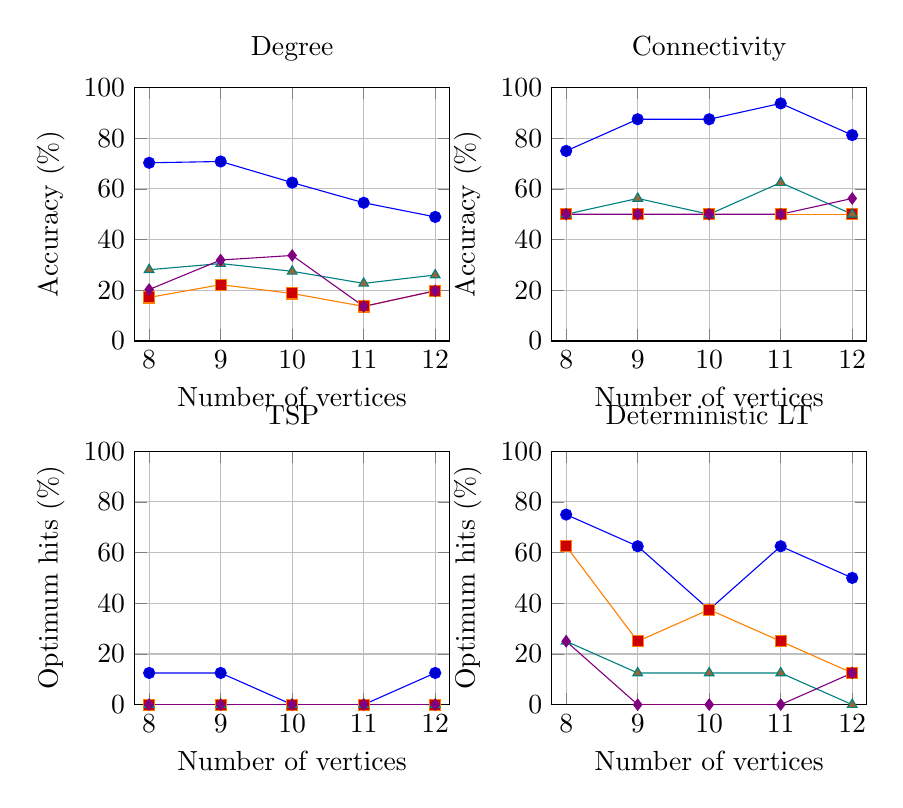
\begin{tikzpicture}
\begin{groupplot}[group style={group size=2 by 2,horizontal sep=1.3cm,vertical sep=1.4cm},
width=.46\textwidth,height=4.8cm,xlabel={Number of vertices},
xmin=7.8,xmax=12.2,xtick={8,9,10,11,12},ymin=0,ymax=100,grid=major,
legend style={font=\scriptsize},legend columns=2]
\nextgroupplot[title={Degree},ylabel={Accuracy (\%)},legend to name=modellegend]
\addplot+[blue,mark=*] coordinates {(8,70.31250000) (9,70.83333333) (10,62.50000000) (11,54.54545455) (12,48.95833333)};
\addlegendentry{Jev action}
\addplot+[orange,mark=square*] coordinates {(8,17.18750000) (9,22.22222222) (10,18.75000000) (11,13.63636364) (12,19.79166667)};
\addlegendentry{4B grammar}
\addplot+[teal,mark=triangle*] coordinates {(8,28.12500000) (9,30.55555556) (10,27.50000000) (11,22.72727273) (12,26.04166667)};
\addlegendentry{9B grammar}
\addplot+[violet,mark=diamond*] coordinates {(8,20.31250000) (9,31.94444444) (10,33.75000000) (11,13.63636364) (12,19.79166667)};
\addlegendentry{4B scores}
\nextgroupplot[title={Connectivity},ylabel={Accuracy (\%)}]
\addplot+[blue,mark=*] coordinates {(8,75.00000000) (9,87.50000000) (10,87.50000000) (11,93.75000000) (12,81.25000000)};
\addplot+[orange,mark=square*] coordinates {(8,50.00000000) (9,50.00000000) (10,50.00000000) (11,50.00000000) (12,50.00000000)};
\addplot+[teal,mark=triangle*] coordinates {(8,50.00000000) (9,56.25000000) (10,50.00000000) (11,62.50000000) (12,50.00000000)};
\addplot+[violet,mark=diamond*] coordinates {(8,50.00000000) (9,50.00000000) (10,50.00000000) (11,50.00000000) (12,56.25000000)};
\nextgroupplot[title={TSP},ylabel={Optimum hits (\%)}]
\addplot+[blue,mark=*] coordinates {(8,12.50000000) (9,12.50000000) (10,0.00000000) (11,0.00000000) (12,12.50000000)};
\addplot+[orange,mark=square*] coordinates {(8,0.00000000) (9,0.00000000) (10,0.00000000) (11,0.00000000) (12,0.00000000)};
\addplot+[teal,mark=triangle*] coordinates {(8,0.00000000) (9,0.00000000) (10,0.00000000) (11,0.00000000) (12,0.00000000)};
\addplot+[violet,mark=diamond*] coordinates {(8,0.00000000) (9,0.00000000) (10,0.00000000) (11,0.00000000) (12,0.00000000)};
\nextgroupplot[title={Deterministic LT},ylabel={Optimum hits (\%)}]
\addplot+[blue,mark=*] coordinates {(8,75.00000000) (9,62.50000000) (10,37.50000000) (11,62.50000000) (12,50.00000000)};
\addplot+[orange,mark=square*] coordinates {(8,62.50000000) (9,25.00000000) (10,37.50000000) (11,25.00000000) (12,12.50000000)};
\addplot+[teal,mark=triangle*] coordinates {(8,25.00000000) (9,12.50000000) (10,12.50000000) (11,12.50000000) (12,0.00000000)};
\addplot+[violet,mark=diamond*] coordinates {(8,25.00000000) (9,0.00000000) (10,0.00000000) (11,0.00000000) (12,12.50000000)};
\end{groupplot}
\end{tikzpicture}
\par\ref{modellegend}

\caption{Selected size curves on the structural challenge. Exact-task
accuracy and construction optimum-hit rate are different metrics. Each
construction point has eight episodes; curves do not imply monotone or
size-causal difficulty. Full task/size counts are in the artifact.}
\label{fig:size}
\end{figure}

\subsection{Legal construction does not imply competitive optimization}
\begin{table}[t]
\centering\small
\begin{tabular}{lrrrrr}
\toprule
Task & Jev action & 4B grammar & 9B grammar & 4B scores & Classical \\
\midrule
MaxCut & 0/40 & 0/40 & 0/40 & 0/40 & 29/40 \\
TSP & 3/40 & 0/40 & 0/40 & 0/40 & 37/40 \\
Deterministic LT & 23/40 & 13/40 & 5/40 & 3/40 & 35/40 \\
Modularity & 7/40 & 0/40 & 0/40 & 0/40 & 35/40 \\
\bottomrule
\end{tabular}

\caption{Optimal solutions over forty scheduled episodes per construction
task. Classical references use separate revisable full-solution algorithms.
All model episodes in this table are feasible.}
\label{tab:optimal}
\end{table}
\begin{table}[t]
\centering\small
\resizebox{\textwidth}{!}{\begin{tabular}{lrrrrrr}
\toprule
Task & Jev action & 4B grammar & 9B grammar & 4B scores & Classical & Uniform \\
\midrule
MaxCut & 8.150 & 11.125 & 11.050 & 9.200 & 0.450 & 5.325 \\
TSP & 45.850 & 338.150 & 306.450 & 351.000 & 0.200 & 331.288 \\
Deterministic LT & 0.600 & 2.625 & 3.725 & 4.125 & 0.175 & 4.182 \\
Modularity & 0.169 & 0.290 & 0.320 & 0.281 & 0.007 & 0.338 \\
\bottomrule
\end{tabular}
}
\caption{Mean additive objective gap, lower is better. Uniform is the exact
expected gap of uniform legal decisions, not a sampled solver. Columns are
comparable within a row only; the four objectives have different units.}
\label{tab:gaps}
\end{table}

All four primary bounded configurations miss every MaxCut optimum; their mean gaps also
exceed the uniform-policy expected gap (Table~\ref{tab:gaps}). Classical cut
search reaches 29/40 optima. For TSP, Jev reaches 3/40 optima versus
37/40 for nearest-neighbor plus 2-opt. Thus neither legal output nor relative
improvement over a weak neural configuration implies a useful solver.
On LT, 4B scoring attains only 3/40 optima versus 13/40 for 4B generation;
the same readout that improves adjacency can harm sequential performance.

The suspicious cut and modularity floors triggered independent NetworkX
objective recomputation, with zero mismatches. The 4B grammar configuration
assigns every remaining vertex to B in all forty cuts; 9B does so in 39/40,
scoring in 20/40, and Jev in 13/40. The scoring method chooses all-A on every
modularity episode, legally obtaining $Q=0$. These are observed policies, not
proofs of an internal failure mechanism or an exhaustive absence of bugs.

\subsection{Where actual trajectories lose optimality}
\label{sec:regret}
Let $s_t$ include all choices through time $t$, and let $V(s_t)$ be the best
final objective still reachable by any legal completion. Define
\[
 r_t =
 \begin{cases}
 V(s_{t-1})-V(s_t), & \text{maximization},\\
 V(s_t)-V(s_{t-1}), & \text{minimization}.
 \end{cases}
\]
Restricting the completion set cannot improve the optimum, so $r_t\geq0$.
For a complete trajectory, $V(s_0)=f^\star$ and $V(s_T)=f$; consequently
$\sum_{t=1}^T r_t=\gap$. This elementary telescoping identity distinguishes
the first irreversible loss from a later locally optimal action in an already
damaged state. It does not require one unique optimal action.

We compute this diagnostic \emph{after inference} from actual histories,
using exact prefix-conditioned continuations. Across 640 complete
construction episodes and 4,480 decisions, every decomposition equals the
independently replayed final gap within $10^{-12}$.
Table~\ref{tab:loss} shows how often optimality is lost immediately.
For MaxCut, only 7--8 of forty episodes lose optimality at the first action
despite every complete neural solution being suboptimal. In TSP, the first
action already loses optimality in 22/40 grammar-4B and 29/40 scoring episodes,
versus 3/40 for Jev. No oracle continuation value was returned to the model.

\begin{table}[t]
\centering\small
\begin{tabular}{lrrrr}
\toprule
Task & Jev action & 4B grammar & 9B grammar & 4B scores \\
\midrule
MaxCut & 8/40 & 8/40 & 8/40 & 7/40 \\
TSP & 3/40 & 22/40 & 21/40 & 29/40 \\
Deterministic LT & 8/40 & 12/40 & 24/40 & 26/40 \\
Modularity & 12/40 & 10/40 & 23/40 & 23/40 \\
\bottomrule
\end{tabular}

\caption{Episodes losing every globally optimal completion at the first
decision, over all forty feasible episodes. Later errors remain represented
in the full per-step regret artifact. This is a retrospective diagnostic,
not a new inference experiment.}
\label{tab:loss}
\end{table}

\subsection{Latency and native conformance are separate outcomes}
\begin{table}[t]
\centering\small
\begin{tabular}{lrr}
\toprule
Method & Median (ms) & p95 (ms) \\
\midrule
Jev action & 70.01 & 115.55 \\
4B grammar & 94.24 & 146.18 \\
9B grammar & 148.64 & 235.12 \\
4B scores & 64.41 & 139.83 \\
\bottomrule
\end{tabular}

\caption{Observed client-path request latency on the challenge. Network,
rendering, cache and hosting differ; this is not an architecture-isolated
speed comparison. No compute-equivalence claim is made.}
\label{tab:latency}
\end{table}
Across development and challenge, the four-method matrix makes 10,352
actual calls for 5,264 scheduled instance evaluations. Jev retains 25 strict
native observations: 24 probability-sum checks and one choice/argmax check.
All supplied actions are eligible under the separately frozen action protocol.
We neither normalize probabilities nor infer replacement choices.
The unchanged strict production parser and its historical results remain
available as a different protocol.

The challenge scoring method evaluates 8,880 candidates in 1,920 prefixes,
with 1,920 unused generated tokens. Median request latency is 64.41 ms,
compared with Jev's 70.01 ms (Table~\ref{tab:latency}). This is not evidence
that one architecture is inherently faster. Vendor-reported tokens are
preserved but are not interchangeable autoregressive steps, FLOPs, energy,
or monetary cost. No unsupported carbon or cost saving is inferred.

\section{Prospective new-seed confirmation}
\label{sec:confirmation}
After fixing the common-interface protocol and four configurations, we
registered a separate confirmation before generating or evaluating its
graphs. Seed 20261012, sizes 8--12, eight repetitions and the same 128-proposal
cap were fixed. The prior pool includes the earlier exclusion pool, both
inspected development banks, the original challenge, and forty executed
TSP confirmation metrics: 2,052 labeled normalized graph records after
deduplication. These are not 2,052 isomorphism classes.
Independent graph reconstruction and 1,421 exact VF2 comparisons after
necessary invariant screening found zero prior overlaps.

The generator fills 952/960 requested instances. Four cycle pairs at $n=8$
exhaust the finite proposal budget, leaving eight explicitly missing cases;
cycle has 72 instances and every other task reaches its quota.
The seed is not retried and no unmatched fallback is introduced.
This limitation affects coverage and precision, not just implementation
bookkeeping: only four cycle-pair clusters remain at $n=8$.
The repeated task/size quotas are not changed after observing any model answer.

All four methods complete all 952 realized cases, using 1,912 calls each:
3,808 instance evaluations and 7,648 actual calls. The eight Jev
probability-sum observations remain conformance diagnostics; no action
execution fails. Sealed attempts, scores and requests replay successfully,
and initial public requests agree across all methods. The same diagnostic
exporter checks another 640 construction trajectories and 4,480 decisions,
again with zero continuation-loss telescoping mismatches.

\begin{table}[t]
\centering\small
\begin{tabular}{lrrrr}
\toprule
Exact task (macro \%) & Jev action & 4B grammar & 9B grammar & 4B scores \\
\midrule
Adjacency & 100.00 & 63.75 & 58.75 & 85.00 \\
Degree & 64.15 & 17.38 & 25.73 & 20.26 \\
Cycle & 71.25 & 51.25 & 53.75 & 50.00 \\
Connectivity & 87.50 & 50.00 & 55.00 & 53.75 \\
Distance & 58.75 & 50.00 & 57.50 & 50.00 \\
Articulation & 58.75 & 50.00 & 50.00 & 50.00 \\
\bottomrule
\end{tabular}

\caption{Prospective confirmation exact macro-size accuracy (\%).
Cycle has 72 cases, degree 400, and the other binary tasks eighty each.
The macro estimator weights the five sizes equally, not by their case counts.}
\label{tab:confirm-exact}
\end{table}
\begin{table}[t]
\centering\small
\begin{tabular}{lrrrrr}
\toprule
Task & Jev action & 4B grammar & 9B grammar & 4B scores & Classical \\
\midrule
MaxCut & 0/40 & 0/40 & 0/40 & 0/40 & 20/40 \\
TSP & 2/40 & 0/40 & 0/40 & 0/40 & 40/40 \\
Deterministic LT & 21/40 & 6/40 & 2/40 & 2/40 & 34/40 \\
Modularity & 2/40 & 0/40 & 0/40 & 0/40 & 34/40 \\
\bottomrule
\end{tabular}

\caption{Prospective confirmation optimal solutions over forty scheduled
episodes per construction. All episodes are feasible; classical algorithms
are independently recomputed on these new graphs.}
\label{tab:confirm-optimal}
\end{table}
\begin{table}[t]
\centering\small
\resizebox{\textwidth}{!}{\begin{tabular}{lrrrrrr}
\toprule
Task & Jev action & 4B grammar & 9B grammar & 4B scores & Classical & Uniform \\
\midrule
MaxCut & 9.000 & 11.575 & 11.375 & 9.825 & 0.725 & 5.475 \\
TSP & 45.300 & 315.950 & 298.250 & 345.100 & 0.000 & 334.111 \\
Deterministic LT & 0.825 & 2.600 & 3.575 & 3.425 & 0.250 & 3.677 \\
Modularity & 0.209 & 0.290 & 0.294 & 0.269 & 0.005 & 0.326 \\
\bottomrule
\end{tabular}
}
\caption{Prospective confirmation mean additive gaps. Uniform columns are
exact policy expectations. No graph, task or method is selected for inclusion
based on its observed score.}
\label{tab:confirm-gap}
\end{table}

The confirmation preserves the principal qualitative observations without
reproducing every numerical ranking. Jev retains its adjacency ceiling;
4B scoring again improves adjacency over 4B grammar (85\% versus 63.75\%).
All methods again miss every MaxCut optimum and have larger expected
gap than the uniform legal policy. TSP optimum hits are 2/40 for Jev,
zero for the other neural configurations, and 40/40 for the classical
reference. Such a classical ceiling is evidence that these particular small
TSP instances are controls for neural interfaces, not difficult classical
optimization benchmarks. On LT, scoring reaches 2/40 optima versus 6/40
for 4B grammar, retaining the task-dependent tradeoff.

Conversely, 9B distance accuracy changes from 42.5\% on the inspected bank to
57.5\% here; an individual ranking from one small sample is not a universal
capacity claim. Jev-minus-4B-grammar articulation accuracy is 8.75 percentage
points with pointwise interval [0,17.5], not a separately established
family-wise significant improvement. Full paired intervals appear in the
appendix. This confirmation addresses reuse of inspected graphs, but not
unseen generator families, larger sizes, pretraining contamination or
closed-model service drift.

\section{Interface controls and stronger-model context}
\label{sec:controls}
\paragraph{Graph-preserving presentation changes.}
We preregistered 120 exact-task cases from the confirmation bank: four per
task and size. Binary tasks use two complete query/construction pairs;
degree uses four prespecified degree strata, not every class. Original,
identical-repeat, node-relabeling, edge-shuffling and option-reversal arms
produce 2,400 decisions across the four methods. Independent NetworkX checks
preserve every transformed label. The relabeling consistently transforms
queries and edge endpoints without also shuffling edge positions.
Two edge permutations leave the actual serialized input unchanged; both
are retained and identified rather than replaced.

All actions are valid. Four Jev strict-native observations are retained
separately. Adjacency remains robust for Jev on all twenty selected cases,
but its degree correctness falls from 15/20 in the original arm to 11/20
after relabeling; only 9/20 are correct across all five arms
(Table~\ref{tab:robust}). An identical repeat already changes two Jev
degree choices, so individual flips cannot all be causally attributed to
the intervention.

Conversely, 4B grammar connectivity chooses the same answer across all five
arms on every case, yet is consistently wrong on ten of twenty cases.
For 9B articulation, original and reversed-option accuracy are both 10/20,
yet reversing options flips all twenty semantic choices; identical repeats,
relabeling and edge shuffling flip none. No case is correct across all five
arms. Marginal accuracy can therefore
hide severe semantic-choice instability; invariant wrong output is not
successful robustness. This is a finite descriptive panel with dependent
query pairs, one repeat, and fixed arm ordering, not a population guarantee
or a comparison over 600 independent graphs per method.

\begin{table}[t]
\centering\small
\begin{tabular}{lrrrr}
\toprule
Task & Jev action & 4B grammar & 9B grammar & 4B scores \\
\midrule
Adjacency & 20/20 & 10/20 & 11/20 & 8/20 \\
Degree & 9/20 & 1/20 & 3/20 & 3/20 \\
Cycle & 9/20 & 4/20 & 10/20 & 10/20 \\
Connectivity & 13/20 & 10/20 & 10/20 & 8/20 \\
Distance & 10/20 & 10/20 & 5/20 & 0/20 \\
Articulation & 9/20 & 1/20 & 0/20 & 0/20 \\
\bottomrule
\end{tabular}

\caption{Cases correct in all five presentation arms, over twenty selected
cases per task. Full arm accuracies and paired choice-flip counts appear in
the appendix. The degree panel uses four prespecified degree strata per size.}
\label{tab:robust}
\end{table}

\paragraph{Isolating the readout at a fixed token prefix.}
The main 4B comparison changes rendering, label coding and decoding, not
only the mathematical selection rule. To test the latter directly, we
registered 100 initial states: two opaque-ID-first cases per task and size
from the completed confirmation bank. Three rotating-order arms use exactly
the same prompt token IDs and candidate tokens: requested candidate scores,
an identical repeat, and candidate-masked greedy one-token generation.
The greedy action is mapped from its actually emitted token; it is not
substituted by a post-hoc argmax. The generated token is ignored only in
the score arms, and all generated tokens are counted.

All 300 calls succeed. Score argmax and greedy generation agree on 100/100
choices, as do the score repeats. The largest conditional-probability
difference is exactly zero in these observed responses. Payload replay checks
identical prefixes, the mask, candidate mapping and token accounting.
This is consistent with the elementary equivalence of greedy selection and
argmax on the same logits; it is not a universal backend equivalence or a
successful CPU SemIf reproduction. In particular, the main adjacency gain
must be described as a \emph{decision-pipeline} effect, not an isolated
benefit of using argmax. Which remaining rendering or coding component causes
that gain is not identified by this control. Construction states here are
initial states only, not new rollout scores.

\paragraph{Teacher-forced controls are not rollout scores.}
On 24 development graphs, 48 informative optimum-prefix states were tested
with original, repeated, reversed-option and explicit-description arms:
384 real decisions across Jev and constrained 9B. Relative to the original,
9B changed 15/48 valid choices under option reversal and 0/48 on identical
repeats; Jev changed 5/46 and 2/46. Repetition variability prevents attributing
every changed choice to the treatment. Both methods solve all six late
MaxCut original-arm states, despite poor free-running cut performance.
This illustrates why favorable oracle-prefix decisions cannot substitute for
own-history episodes.

\paragraph{Prospective probability diagnostics.}
Earlier canonical Jev logs do not retain complete probability vectors,
so their calibration cannot be reconstructed from choices or sum diagnostics.
We instead register new calls on all 792 exact cases of the confirmation
bank, for Jev action and 4B candidate scores: 1,584 observations.
Raw vector entries are neither normalized nor clipped. Probability scores
require action eligibility, exact option keys, finite entries in $[0,1]$
and mass within the frozen $10^{-6}$ tolerance. Omitted vectors and
all-scheduled action accuracy remain separate outcomes.

For accepted vectors, summed multiclass Brier loss is
$\sum_k(p_k-\mathbf{1}[k=y])^2$ and logarithmic loss is $-\log p_y$.
A zero true-label probability has positive-infinite loss; it is not replaced
by a small epsilon or silently dropped from an average. Binary uniform
Brier is therefore $0.5$ under this summed convention, not $0.25$.
We compare both models and the uniform reference only on the common-valid
intersection, alongside each model's own retained-vector count.
Five fixed reliability bins use the probability of the \emph{actually
supplied choice}, not an inferred replacement argmax or an assumed interpretation
of a vendor confidence scalar. No calibration parameter or threshold is fitted.
These are row-averaged, task-specific diagnostics on inspected synthetic
graphs, not population calibration guarantees.

All 792 actions per method are eligible. Jev retains 774 vectors after
eighteen sum-invalid degree vectors are omitted; both choice/argmax-disagreeing
vectors are retained with the actual supplied choices. All 792 token-score
vectors are valid, giving 774 common-valid rows across tasks.
Despite Jev's above-chance action accuracy on distance (48/80) and articulation
(47/80), their Brier losses, 0.509155 and 0.508225, exceed the uniform
reference of 0.5; their logarithmic losses also exceed $\log 2$.
Thus accuracy above chance and numeric probability output do not establish
useful uncertainty estimates. In contrast, Jev's adjacency Brier is
0.000120. The task-specific pattern, not a pooled calibration ranking, is
the intended diagnostic.

\begin{table}[t]
\centering\small
\begin{tabular}{lrrrrr}
\toprule
Task & Valid J/T & Common & Jev & 4B scores & Uniform \\
\midrule
Adjacency & 80/80 & 80 & 0.000 & 0.199 & 0.500 \\
Degree & 382/400 & 382 & 0.458 & 0.841 & 0.900 \\
Cycle & 72/72 & 72 & 0.420 & 0.720 & 0.500 \\
Connectivity & 80/80 & 80 & 0.152 & 0.682 & 0.500 \\
Distance & 80/80 & 80 & 0.509 & 0.550 & 0.500 \\
Articulation & 80/80 & 80 & 0.508 & 0.534 & 0.500 \\
\bottomrule
\end{tabular}

\caption{Prospective probability audit: summed multiclass Brier, lower is
better. ``Valid J/T'' gives each method's own vector denominator; loss
columns use exactly the common-valid rows. Uniform is evaluated on the same
rows with their actual option cardinalities. No cross-task aggregate is used.}
\label{tab:brier}
\end{table}

This audit also exposed a bookkeeping bug after inference: canonical JSON
key sorting changed the order of floating-point additions. Ten native
sum metadata values differed on replay by at most $2.22\times10^{-16}$,
although no vector's eligibility changed. The original producer failed to
seal its native lane; all 792 recorded responses were retained without
additional calls. Corrected offline analysis is separately versioned and
preserves the original failure, vectors and action decisions.
Its derived-sum roundoff check is distinct from both the unchanged $10^{-6}$
vector gate and the failed $0.01$ CPU/GPU reproduction criterion.

\paragraph{A prospective TSP wording confirmation.}
Six late Jev TSP control failures all selected the city closest to start
vertex 0, although the actual current endpoint differed. Independent
enumeration confirmed the labels. This motivated a bundled state-explicit
wording treatment, not a claim to identify an internal mechanism.

Forty newly generated weighted metrics were independently excluded from
eighty earlier weighted TSP instances within a refreshed 1,840-record pool.
Under the original strict protocol, Jev completes 36/40 original-wording
and 33/40 explicit-wording episodes. On the 29 commonly feasible graphs,
relative gap improves by 0.3761 (pointwise 95\% interval [0.2337, 0.5462]);
this conditional comparison does not establish improved completion.

A separately registered action-observation run on those same forty metrics
completes all eighty episodes. Mean relative gap falls from 0.5152 to 0.1603;
the paired reduction is 0.3550 [0.2463, 0.4729]. Nine strict-native observations
remain recorded. This second protocol removes feasibility selection within
that comparison, but is a repeated use of the metrics, not a second untouched
confirmation set. No prior failed response was retrospectively rescued.

\paragraph{Stronger reasoning models change the picture.}
Completed earlier \emph{seven-task, legacy-protocol development} runs provide
an important counterpoint. GPT-5.4 solves all 200 exact decisions and all 62
feasibly completed construction episodes optimally; two timeouts leave
two other constructions incomplete (559 actual calls). GPT-6-Astra solves
all 200 exact decisions and 63/64 constructions optimally with no failures
(576 calls); its single suboptimal cut has value 20 versus optimum 21.
These are not missing columns to paste into the common-interface challenge:
the tasks, bank and protocol differ. They nevertheless preclude interpreting
weak bounded Qwen results as evidence of universal LLM incapacity.

The subsequently completed \emph{ten-task legacy-interface Astra challenge}
uses the same 960 graph instances and references as the inspected canonical
challenge. Its frozen runner replays all 1,920 calls with no failures.
All 800 exact decisions are correct, and 159/160 constructions are optimal
(Table~\ref{tab:astra-legacy}). The sole miss is an eight-vertex community
partition with $Q=0.0244444$ versus $Q^\star=0.08$; independent NetworkX
evaluation confirms all forty community objectives, and enumeration of all
128 anchored assignments confirms this optimum.

This result is intentionally separate from the primary matrix: the legacy
instructions and option descriptions differ, with zero of 960 full initial
requests identical to their canonical counterparts. Astra uses default
reasoning and a 4,096-token ceiling rather than the bounded local decoding
settings. The result demonstrates that these graph instances are tractable
for this stronger configuration; it does not isolate model architecture,
protocol effects or equal-compute superiority.

\begin{table}[t]
\centering\small
\begin{tabular}{lrrr}
\toprule
Task & Correct / optimal & Feasible & Mean gap \\
\midrule
Adjacency & 80/80 & 80/80 & -- \\
Degree & 400/400 & 400/400 & -- \\
Cycle & 80/80 & 80/80 & -- \\
Connectivity & 80/80 & 80/80 & -- \\
Distance & 80/80 & 80/80 & -- \\
Articulation & 80/80 & 80/80 & -- \\
MaxCut & 40/40 & 40/40 & 0.000000 \\
TSP & 40/40 & 40/40 & 0.000000 \\
Deterministic LT & 40/40 & 40/40 & 0.000000 \\
Modularity & 39/40 & 40/40 & 0.001389 \\
\bottomrule
\end{tabular}

\caption{Completed Astra legacy-interface challenge on the same graphs as
the inspected primary challenge. The first six rows report correct answers;
the final four report optimum hits. Mean gaps are task-specific and are not
pooled. This is a separate protocol/default-reasoning reference, not an
additional column of the canonical four-method matrix.}
\label{tab:astra-legacy}
\end{table}

\subsection{Completed canonical GPT-5.4 anchor}
This separately registered tool-free, default-reasoning GPT-5.4 run uses
the identical canonical structural-challenge requests and own histories.
It made 1,840 actual calls, with 9 failed attempts.
Failures remain in scheduled denominators; no retry or repair was performed.
\begin{table}[ht]\centering\small
\begin{tabular}{lrrr}
\toprule
Exact task & GPT-5.4 (\%) & Jev (\%) & 95\% interval (pp) \\
\midrule
Adjacency & 100.00 & 100.00 & [0.00, 0.00] \\
Degree & 100.00 & 61.43 & [33.75, 43.30] \\
Cycle & 100.00 & 66.25 & [27.50, 40.00] \\
Connectivity & 100.00 & 85.00 & [8.75, 22.50] \\
Distance & 100.00 & 58.75 & [35.00, 46.25] \\
Articulation & 100.00 & 65.00 & [26.25, 43.75] \\
\bottomrule
\end{tabular}

\caption{Canonical exact macro-size accuracy. Intervals are paired,
size-stratified pointwise GPT-minus-Jev differences, not family-wise tests.}
\end{table}
\begin{table}[ht]\centering\small
\begin{tabular}{lrrrr}
\toprule
Task & GPT feasible & GPT optima & Jev optima & GPT gap \\
\midrule
MaxCut & 36/40 & 36/40 & 0/40 & 0.000 \\
TSP & 39/40 & 39/40 & 3/40 & 0.000 \\
Deterministic LT & 40/40 & 40/40 & 23/40 & 0.000 \\
Modularity & 36/40 & 36/40 & 7/40 & 0.000 \\
\bottomrule
\end{tabular}

\caption{Canonical construction results. Gaps condition on GPT feasible
completion and have different units across rows; they are not a pooled score.}
\end{table}
Observed median/p95 GPT request latency was 7220.20/96561.70 ms.
Reasoning budget and hosting differ from the small no-thinking local baselines.
These are inspected-bank common-protocol anchors, not the prospective new-seed
confirmation or a matched-compute architectural comparison.

Request identity here concerns all 960 initial public requests. Later
construction requests follow each method's own choices and need not match;
neither model receives the other's trajectory or oracle actions.
All nine failed attempts are timeouts in construction episodes: four MaxCut,
one TSP and four modularity. Across 960 scheduled episodes, all 800 exact
answers are correct and all 151 feasible constructions attain exact optima.
An additional independent objective check reproduces every feasible
construction using NetworkX or exact-rational diffusion. This strengthens
the interpretation that the bounded models' failures are not unavoidable
properties of the graph instances or the canonical action interface.
It does not establish equal-compute superiority, out-of-distribution
generalization, or unconditional construction perfection: the nine incomplete
episodes remain in every all-scheduled denominator.

\paragraph{Exploratory larger-local-model check.}
After inspecting the primary results, we registered a small, score-blind
selection from the confirmation bank: four cases per exact task and two per
construction at each of $n=8,12$, retaining binary pairs and degree strata.
The resulting 64-episode, 160-decision panel compares a fresh Qwen3.5-27B
BF16 run with reused Jev and bounded-Qwen reference traces on exactly the
same instances. The 27B configuration keeps the 64-token, no-thinking,
legal-choice grammar contract and completes every episode without failure.
This is an inspected-bank exploratory extension, not an independent replication.

On this panel Jev exceeds bounded 27B on degree (6/8 versus 4/8), connectivity
(7/8 versus 6/8), and cycle detection (5/8 versus 4/8), while 27B exceeds Jev
on distance (5/8 versus 4/8). Adjacency and articulation tie
(Appendix~\ref{app:larger-local}). Jev has better mean cut, TSP and community
objectives; LT ties, including 2/4 optimum hits for both. Neither reaches
any cut, TSP or community optimum on these four-case tasks.
These observations concern the specified no-thinking grammar configuration
only. They do not establish parameter equivalence or bound 27B's unrestricted
capacity; the completed thinking comparison below substantially changes the
exact-task interpretation. Historical reference latency is not a controlled
timing comparison, and these small denominators support no significance claim.

\paragraph{Thinking improves exact answers but exposes deadline failures.}
The completed 27B and 9B thinking lanes use the same selected instances and
canonical initial requests, but enable thinking, remove grammar constraints,
and raise the output-token cap from 64 to 8,192 jointly. The per-request
deadline is 180 seconds. Their exact counts are \EPLargeThinkingExact{} and
\EPSmallThinkingExact{}, versus \EPJevExact{} for reused Jev and
\EPGrammarExact{} for 27B grammar. Every returned exact answer is correct:
\EPLargeThinkingReturned/\EPLargeThinkingReturned{} and
\EPSmallThinkingReturned/\EPSmallThinkingReturned{}, respectively. The
remaining exact cases are timeouts, not observed wrong predictions; 27B's
one timeout is a distance query. All 48 scheduled exact cases remain in
the reported accuracy denominators.

Both thinking lanes time out within every one of their sixteen construction
episodes, leaving zero feasible constructions. Across the whole panel, 27B
records \EPLargeThinkingFailures{} timed-out calls among
\EPLargeThinkingCalls{} attempts; 9B records \EPSmallThinkingFailures{}
among \EPSmallThinkingCalls{}. Conditional construction gaps are therefore
undefined, not zero, and provide no quality ranking between these
configurations and methods that finish. The substantially stronger exact
results overturn an interpretation of the bounded comparison as
Jev--27B capability equivalence. This is a joint inference-configuration
effect, not an isolated causal effect of reasoning.

A separate timeout-only 9B control raises the deadline to 600 seconds while
retaining the 8,192-token cap. All sixteen construction attempts then terminate
at that token cap, still yielding no feasible trajectories
(Table~\ref{tab:deadline-control}). Increasing wall time alone therefore does
not resolve these completion failures.

\paragraph{Two additional trained decision readouts.}
We also evaluate the released Decider-2B v11 and Kev-4B trained inference
paths \cite{decider2026model,decider2026code,kev2026model,kev2026code},
not ordinary next-token substitutes. Both complete all 64 episodes in
160 calls, without execution failures. Decider obtains \EPDeciderExact{}
exact answers and Kev \EPKevExact{}, versus \EPJevExact{} for Jev.
Neither answers a degree query correctly, despite legal, varied predictions
and the full eight- or twelve-class vocabulary. Decider reaches no construction
optimum; Kev reaches one LT optimum, compared with Jev's two LT optima.
This is not an all-task Jev win: Kev's mean modularity gap is
\EPKevCommunityGap{}, better than Jev's \EPJevCommunityGap{}.
Appendix~\ref{app:larger-local} reports taskwise coverage, optimum hits and
conditional gaps separately, along with dtype, source-version and environment
limitations. Native probability conformance is not evidence of calibration
on these graph tasks.

\paragraph{An encoder-based trained decision model.}
A separate Laya typed-decisions pilot evaluates a roughly 421M-parameter
ModernBERT encoder with its genuine trained choice head \cite{laya2026},
using native CPU FP32 inference on the same 64-case panel.
Its checkpoint contract permits 1,024 total tokens and a 256-token head.
Lossless tokenization checks reject two $n=12$ LT requests before inference;
no graph, question or option is truncated. The remaining 62 episodes require
156 successful forwards, with no later context overflow.
Laya obtains 22/48 exact answers versus 33/48 for reused Jev, and no optimal
construction among fourteen initially supported cases versus two for Jev.
All forty binary answers are \texttt{yes}, yielding the constant-yes baseline
of 20/40; degree contributes 2/8. Native logits, probability-to-ID mapping
and canonical action replay are checked rather than assuming these constant
predictions are a parser failure. A separate twenty-call option-order
diagnostic preserves \texttt{yes} on all ten paired states after reversal,
arguing against a fixed-first-option explanation on this selected subset,
not establishing a claim about every Laya prompt or task.
Appendix~\ref{app:laya} separates input coverage from solution quality and
discloses an offline postprocessing recovery.

\section{Exact contracts, invariants and budgets}
\label{app:contracts}
Node relabeling does not change truth, but rendering may affect model outputs.
Cycle twins match degree sequences, not component count: $m>n-c(G)$ is an
exact cycle test for the stated undirected contract. Distance pairs share
their threshold and finite distances $h,h+1$. Articulation compares total
component counts before and after deletion; isolated vertices are not
articulation points under this definition.

For LT, normalized incoming weights and a fixed one-half threshold are applied
synchronously to the two initially chosen seeds. Seeds are not activated one
at a time with diffusion between selections. For TSP, prefix cost, the current
endpoint, all remaining cities, and final return to 0 enter continuation
values. For partitions, vertex 0 fixes complement symmetry without excluding
any attainable objective; empty sides remain legal. Modularity search is over
at most two groups, including one group. Histories must contain legal,
exact-string action IDs, not a repaired subset of malformed model output.

Reference values are obtained by exhaustive partitions/seed pairs or exact
TSP dynamic programming and checked independently. Uniform cut expectation is
$m/2$; uniform TSP expectation is $2\sum_{\{u,v\}}d_{uv}/(n-1)$.
Uniform LT averages all distinct unordered seed pairs. For uniform binary
modularity with one fixed vertex, expected modularity is
$-\sum_v d_v^2/(8m^2)$. These are expectations of random legal policies,
not attainable objective guarantees for one particular rollout.

\paragraph{Why the LT guarantee cannot be imported.}
Consider vertices $a,b,d,c$ with edges $a\to c$, $b\to c$, $d\to c$.
Each edge has weight $1/3$ and $c$ requires at least two active parents.
Writing $\sigma(S)$ for final spread including seeds,
$\sigma(\varnothing)=0$, $\sigma(\{a\})=\sigma(\{b\})=1$, and
$\sigma(\{a,b\})=3$. The marginal gain of adding $b$ is 1 at the empty set
but 2 at $\{a\}$, violating diminishing returns. This four-vertex example
uses the benchmark's exact deterministic diffusion semantics and illustrates
why the randomized-threshold theorem does not apply.

\section{Paired uncertainty for the inspected matrix}
\centering
\begin{tabular}{lrrr}
\toprule
Task & $\Delta$ (pp) & Pointwise 95\% interval & Clusters \\
\midrule
Adjacency & 40.00 & [33.75, 46.25] & 40 \\
Degree & 43.11 & [37.46, 48.88] & 400 \\
Cycle & 11.25 & [2.50, 18.75] & 40 \\
Connectivity & 35.00 & [27.50, 41.25] & 40 \\
Distance & 8.75 & [3.75, 15.00] & 40 \\
Articulation & 15.00 & [6.25, 23.75] & 40 \\
MaxCut & 0.00 & [0.00, 0.00] & 40 \\
TSP & 7.50 & [0.00, 15.00] & 40 \\
Deterministic LT & 25.00 & [5.00, 42.50] & 40 \\
Modularity & 17.50 & [7.50, 30.00] & 40 \\
\bottomrule
\end{tabular}

\par\raggedright
\smallskip
Differences are Jev action minus 4B grammar in percentage points: exact
accuracy for the first six rows and optimum-hit rate for the last four.
Resampling uses paired identity/construction clusters within each size.
Forty clusters means eight per size for these paired binary and optimization
tasks. Degree has 400 clusters. The MaxCut zero-width interval reflects
the observed all-zero optimum-hit difference, not established equivalence
of the underlying models or equal gap quality.

\section{Paired uncertainty for prospective confirmation}
\centering
\begin{tabular}{lrrr}
\toprule
Task & $\Delta$ (pp) & Pointwise 95\% interval & Clusters \\
\midrule
Adjacency & 36.25 & [30.00, 42.50] & 40 \\
Degree & 46.77 & [41.07, 52.73] & 400 \\
Cycle & 20.00 & [10.00, 30.00] & 36 \\
Connectivity & 37.50 & [31.25, 43.75] & 40 \\
Distance & 8.75 & [3.75, 15.00] & 40 \\
Articulation & 8.75 & [0.00, 17.50] & 40 \\
MaxCut & 0.00 & [0.00, 0.00] & 40 \\
TSP & 5.00 & [0.00, 10.00] & 40 \\
Deterministic LT & 37.50 & [22.50, 52.50] & 40 \\
Modularity & 5.00 & [0.00, 12.50] & 40 \\
\bottomrule
\end{tabular}

\par\raggedright
\smallskip
Conventions are the same as the preceding appendix, but these are new graphs
under the pre-inference registration. Cycle has 36 paired clusters, with four
at size 8 and eight at each other size. No missing pair is assigned a
synthetic model prediction. The construction tasks retain forty clusters each.

\section{Presentation-control detail}
\begin{table}[ht]
\centering\scriptsize
\resizebox{\textwidth}{!}{\begin{tabular}{lrrrrrr}
\toprule
Task & Method & Original & Repeat & Relabel & Edges & Options \\
\midrule
Adjacency & Jev action & 20/20 & 20/20 & 20/20 & 20/20 & 20/20 \\
Adjacency & 4B grammar & 14/20 & 14/20 & 12/20 & 13/20 & 19/20 \\
Adjacency & 9B grammar & 12/20 & 12/20 & 14/20 & 13/20 & 14/20 \\
Adjacency & 4B scores & 17/20 & 17/20 & 15/20 & 19/20 & 14/20 \\
Degree & Jev action & 15/20 & 14/20 & 11/20 & 12/20 & 13/20 \\
Degree & 4B grammar & 3/20 & 3/20 & 2/20 & 2/20 & 6/20 \\
Degree & 9B grammar & 9/20 & 9/20 & 7/20 & 10/20 & 9/20 \\
Degree & 4B scores & 8/20 & 8/20 & 6/20 & 7/20 & 10/20 \\
Cycle & Jev action & 15/20 & 15/20 & 13/20 & 13/20 & 14/20 \\
Cycle & 4B grammar & 10/20 & 10/20 & 10/20 & 10/20 & 10/20 \\
Cycle & 9B grammar & 11/20 & 11/20 & 10/20 & 10/20 & 10/20 \\
Cycle & 4B scores & 10/20 & 10/20 & 10/20 & 10/20 & 11/20 \\
Connectivity & Jev action & 18/20 & 18/20 & 15/20 & 15/20 & 19/20 \\
Connectivity & 4B grammar & 10/20 & 10/20 & 10/20 & 10/20 & 10/20 \\
Connectivity & 9B grammar & 10/20 & 10/20 & 10/20 & 10/20 & 10/20 \\
Connectivity & 4B scores & 10/20 & 10/20 & 10/20 & 10/20 & 9/20 \\
Distance & Jev action & 11/20 & 11/20 & 11/20 & 12/20 & 11/20 \\
Distance & 4B grammar & 10/20 & 10/20 & 10/20 & 10/20 & 10/20 \\
Distance & 9B grammar & 10/20 & 10/20 & 10/20 & 9/20 & 10/20 \\
Distance & 4B scores & 11/20 & 11/20 & 10/20 & 10/20 & 10/20 \\
Articulation & Jev action & 11/20 & 11/20 & 11/20 & 11/20 & 10/20 \\
Articulation & 4B grammar & 10/20 & 10/20 & 10/20 & 10/20 & 10/20 \\
Articulation & 9B grammar & 10/20 & 10/20 & 10/20 & 10/20 & 10/20 \\
Articulation & 4B scores & 10/20 & 10/20 & 10/20 & 10/20 & 10/20 \\
\bottomrule
\end{tabular}
}
\caption{Correct cases / scheduled cases in each arm. Counts are not
independent across arms or paired queries. An unchanged aggregate accuracy
does not imply unchanged semantic choices.}
\end{table}
\begin{table}[ht]
\centering\scriptsize
\begin{tabular}{lrrrrr}
\toprule
Task & Method & Repeat & Relabel & Edges & Options \\
\midrule
Adjacency & Jev action & 0/20 & 0/20 & 0/20 & 0/20 \\
Adjacency & 4B grammar & 0/20 & 2/20 & 3/20 & 7/20 \\
Adjacency & 9B grammar & 0/20 & 4/20 & 3/20 & 2/20 \\
Adjacency & 4B scores & 0/20 & 4/20 & 2/20 & 9/20 \\
Degree & Jev action & 2/20 & 6/20 & 4/20 & 2/20 \\
Degree & 4B grammar & 0/20 & 12/20 & 11/20 & 12/20 \\
Degree & 9B grammar & 0/20 & 13/20 & 6/20 & 9/20 \\
Degree & 4B scores & 0/20 & 13/20 & 6/20 & 14/20 \\
Cycle & Jev action & 0/20 & 4/20 & 4/20 & 3/20 \\
Cycle & 4B grammar & 0/20 & 6/20 & 8/20 & 8/20 \\
Cycle & 9B grammar & 0/20 & 1/20 & 1/20 & 1/20 \\
Cycle & 4B scores & 0/20 & 0/20 & 0/20 & 1/20 \\
Connectivity & Jev action & 0/20 & 5/20 & 3/20 & 1/20 \\
Connectivity & 4B grammar & 0/20 & 0/20 & 0/20 & 0/20 \\
Connectivity & 9B grammar & 0/20 & 0/20 & 0/20 & 0/20 \\
Connectivity & 4B scores & 0/20 & 0/20 & 0/20 & 3/20 \\
Distance & Jev action & 0/20 & 0/20 & 1/20 & 2/20 \\
Distance & 4B grammar & 0/20 & 0/20 & 0/20 & 0/20 \\
Distance & 9B grammar & 0/20 & 6/20 & 7/20 & 6/20 \\
Distance & 4B scores & 0/20 & 5/20 & 7/20 & 13/20 \\
Articulation & Jev action & 2/20 & 2/20 & 0/20 & 1/20 \\
Articulation & 4B grammar & 0/20 & 0/20 & 0/20 & 18/20 \\
Articulation & 9B grammar & 0/20 & 0/20 & 0/20 & 20/20 \\
Articulation & 4B scores & 0/20 & 0/20 & 0/20 & 20/20 \\
\bottomrule
\end{tabular}

\caption{Choice flips relative to the original arm / both-valid pairs.
There are no invalid actions in this completed panel. Edge counts include the
two retained unchanged inputs; their separate strata are in the artifact.}
\end{table}

\section{Probability-loss detail}
\begin{table}[ht]
\centering\small
\begin{tabular}{lrrrr}
\toprule
Task & Common & Jev & 4B scores & Uniform \\
\midrule
Adjacency & 80 & 0.002 & 0.331 & 0.693 \\
Degree & 382 & 0.935 & 2.036 & 2.312 \\
Cycle & 72 & 0.616 & 1.045 & 0.693 \\
Connectivity & 80 & 0.229 & 1.009 & 0.693 \\
Distance & 80 & 0.735 & 0.747 & 0.693 \\
Articulation & 80 & 0.713 & 0.729 & 0.693 \\
\bottomrule
\end{tabular}

\caption{Logarithmic loss on the common-valid rows from
Table~\ref{tab:brier}, in natural-log units. A positive-infinity entry means at
least one true label received exactly zero probability, not a missing value.
Finite-only averaging is not substituted for an infinite loss.}
\end{table}
The artifact includes all five reliability-bin counts and conditional
accuracies for each task and method, along with all-scheduled action accuracy,
own-valid and common-valid denominators. Vector eligibility is not assumed
independent of task difficulty. The 4B vectors are conditional option-logit
scores, not calibrated posterior probabilities by definition.

\section{Completed expanded-model exploratory panel}
\label{app:larger-local}
The selected graphs are reused from the confirmation bank; opaque-ID selection
within prespecified pairs/strata does not make this a new held-out evaluation.
The 27B configurations use tensor parallelism across two RTX A6000s.
Initial public requests are identical across compared configurations, but
provider interfaces differ and subsequent requests follow each method's own
history. The grammar and trained-native lanes complete all selected episodes;
the thinking lanes have the explicit failures below. Each original historical
lane is fully replayed before subsetting. Terminal candidate requests, actions,
all 64 score rows and summaries are independently replayed and hash-attested.
NetworkX/Fraction checks reproduce every feasible construction objective.
The paper builder verifies every export seal and source hash, recomputes the
CSV denominators and metrics, and requires identical reused reference
trajectories across all exports. No failed episode is removed.

\begin{table}[ht]
\centering\small
\begin{tabular}{lrrrrrr}
\toprule
Task & Jev & 27B G & 27B T & 9B T & Decider & Kev \\
\midrule
Adjacency & 8/8 & 8/8 & 8/8 & 8/8 & 7/8 & 7/8 \\
Degree & 6/8 & 4/8 & 8/8 & 7/8 & 0/8 & 0/8 \\
Cycle & 5/8 & 4/8 & 8/8 & 8/8 & 4/8 & 4/8 \\
Connectivity & 7/8 & 6/8 & 8/8 & 7/8 & 4/8 & 4/8 \\
Distance & 4/8 & 5/8 & 7/8 & 7/8 & 5/8 & 5/8 \\
Articulation & 3/8 & 3/8 & 8/8 & 3/8 & 4/8 & 3/8 \\
Exact total & 33/48 & 30/48 & 47/48 & 40/48 & 24/48 & 23/48 \\
\bottomrule
\end{tabular}

\caption{Exact correct/scheduled answers on the same selected panel.
Each task has four cases at each of $n=8,12$.
G denotes the 64-token no-thinking grammar setting; T denotes unconstrained
thinking with an 8,192-token cap and 180-second deadline.
Jev is a reused reference, not fresh inference. Thinking timeouts remain
in the denominators; these are descriptive counts, not a population ranking.}
\label{tab:expanded-exact}
\end{table}
\begin{table}[ht]
\centering\small
\begin{tabular}{lrrrr}
\toprule
Configuration & Scheduled & Failed & Exact returned & Constructed \\
\midrule
Jev & 64 & 0 & 48/48 & 16/16 \\
27B G & 64 & 0 & 48/48 & 16/16 \\
27B T & 64 & 17 & 47/48 & 0/16 \\
9B T & 64 & 24 & 40/48 & 0/16 \\
Decider & 64 & 0 & 48/48 & 16/16 \\
Kev & 64 & 0 & 48/48 & 16/16 \\
\bottomrule
\end{tabular}

\caption{Completion coverage, separate from correctness. ``Failed'' counts
episodes with an execution failure, all timeouts in the two thinking lanes.
``Exact returned'' counts feasible exact episodes, not correct answers.
Every configuration retains all 64 scheduled episodes. All grammar/native
lanes use 160 calls; 27B T and 9B T use 66 and 64, respectively, because
timeouts terminate individual trajectories without retries.}
\label{tab:expanded-coverage}
\end{table}

\begin{table}[ht]
\centering\small
\textbf{Feasible / scheduled}\par\medskip
\begin{tabular}{lrrrrrr}
\toprule
Task & Jev & 27B G & 27B T & 9B T & Decider & Kev \\
\midrule
MaxCut & 4/4 & 4/4 & 0/4 & 0/4 & 4/4 & 4/4 \\
TSP & 4/4 & 4/4 & 0/4 & 0/4 & 4/4 & 4/4 \\
Deterministic LT & 4/4 & 4/4 & 0/4 & 0/4 & 4/4 & 4/4 \\
Modularity & 4/4 & 4/4 & 0/4 & 0/4 & 4/4 & 4/4 \\
\bottomrule
\end{tabular}

\par\medskip\textbf{Optimum hits / scheduled}\par\medskip
\begin{tabular}{lrrrrrr}
\toprule
Task & Jev & 27B G & 27B T & 9B T & Decider & Kev \\
\midrule
MaxCut & 0/4 & 0/4 & 0/4 & 0/4 & 0/4 & 0/4 \\
TSP & 0/4 & 0/4 & 0/4 & 0/4 & 0/4 & 0/4 \\
Deterministic LT & 2/4 & 2/4 & 0/4 & 0/4 & 0/4 & 1/4 \\
Modularity & 0/4 & 0/4 & 0/4 & 0/4 & 0/4 & 0/4 \\
\bottomrule
\end{tabular}

\caption{Four constructions per task (two at each size). Feasibility and
all-scheduled optimum-hit rates are distinct outcomes. The thinking lanes'
0/4 optimum counts arise from zero completed constructions, not four observed
suboptimal solutions. Labels follow Table~\ref{tab:expanded-exact}.}
\label{tab:expanded-construction}
\end{table}
\begin{table}[ht]
\centering\small
\begin{tabular}{lrrrrrr}
\toprule
Task & Jev & 27B G & 27B T & 9B T & Decider & Kev \\
\midrule
MaxCut & 8.25 & 9.00 & \textemdash & \textemdash & 12.25 & 12.25 \\
TSP & 60.50 & 146.00 & \textemdash & \textemdash & 387.50 & 360.00 \\
Deterministic LT & 1.00 & 1.00 & \textemdash & \textemdash & 4.00 & 1.50 \\
Modularity & 0.235880 & 0.305421 & \textemdash & \textemdash & 0.305421 & 0.113657 \\
\bottomrule
\end{tabular}

\caption{Mean absolute objective gap conditional on feasibility, lower being
better. Each numeric cell has four feasible episodes; each dash denotes zero
feasible episodes and an undefined mean, not zero gap.
Units are cut edges, tour cost, active vertices and modularity respectively;
they are never pooled. Kev improves the modularity gap over Jev despite lower
exact-task accuracy.}
\label{tab:expanded-gaps}
\end{table}

\paragraph{Deadline and output-budget interpretation.}
The 8,192-token cap is not a guarantee of that much decoding before the
180-second wall deadline. For example, 21.3 generated tokens/second permits
only about 3,834 tokens in 180 seconds even before other overhead; this
illustrative arithmetic is not a controlled speed comparison. A separately
registered posthoc 9B control has now completed on all sixteen constructions;
only the deadline changes to 600 seconds, with the 8,192-token cap unchanged
(at most 112 calls). All sixteen first-step attempts end with
\texttt{finish\_length}, each recording exactly 8,192 output tokens and
approximately 239 seconds of client-observed latency, below the relaxed
deadline. No response finishes normally, so no action advances a trajectory.
We do not salvage a choice from truncated final content, retry, or raise the
token cap. All sixteen constructions remain infeasible. Thus, under this
registered contract, relaxing the wall deadline exposes a token-limit
failure rather than a feasible solution-quality estimate.
This is not evidence that the model cannot construct solutions under another
prompt, budget or reasoning configuration. Original failures remain unchanged.

\begin{table}[ht]
\centering\small
\begin{tabular}{lrrrr}
\toprule
Task & 180s feasible & 600s feasible & 600s length stops & 600s gap \\
\midrule
MaxCut & 0/4 & 0/4 & 4 & -- \\
TSP & 0/4 & 0/4 & 4 & -- \\
Deterministic LT & 0/4 & 0/4 & 4 & -- \\
Modularity & 0/4 & 0/4 & 4 & -- \\
\bottomrule
\end{tabular}

\caption{Completed timeout-only Qwen9 control on the same sixteen constructions.
All four cases per task remain in denominators. The 180-second arm has
wall-timeout failures; the 600-second arm has token-limit failures.
Conditional objective gaps are undefined in both arms, not zero.}
\label{tab:deadline-control}
\end{table}

\paragraph{Pinned trained methods and compatibility.}
Decider uses its genuine one-pass restricted-letter readout, BF16 weights and
eager inference. The v11 checkpoint requires source version 1.4.0
(commit \texttt{15ab28e8}); its plain-choice temperature is 1.164, not the
global fallback 1.145. Kev uses the pinned upstream pointer head and
LoRA-merged FP32 backbone (source commit \texttt{569ea449}), with temperature
2.406050072164233 and an independently pinned Qwen3.5-4B-Base.
Model-card and code revisions are cited separately
\cite{decider2026model,decider2026code,kev2026model,kev2026code}.
All 34 registered checkpoint/tokenizer/configuration files are hash-checked;
temperatures are independently derived from the Decider configuration and
restricted CPU loading of the Kev head metadata, rather than trusted solely
from GPU runtime claims. Complete requests retain all original semantic
option IDs and descriptions, with an 8,192-token lossless context gate.

The compatible shared runtime uses Python 3.12, Torch 2.13.0, Transformers
5.17.0 and NumPy 2.3.5, with an isolated Accelerate 1.15.0/PEFT 0.21.0 overlay.
These are not the full declared upstream environments: Kev specifies
Torch below 2.9 and NumPy at least 2.5.3, while Decider specifies NumPy below 2.
Unavailable fused kernels use native reference paths. Dtype and deployment
are not matched across methods; no latency ranking or full-environment
reproduction is claimed. Released temperature fitting is not a calibration
guarantee on this selected graph panel.

\paragraph{A limited CPU/GPU numeric check.}
A separate posthoc control, registered before its fresh CPU forwards, repeats
the first $n=8$ adjacency and first $n=12$ degree request for each trained model.
All four forwards pass the fixed gate of maximum absolute probability
difference at most 0.01 plus native-choice agreement. In adjacency/degree order,
the differences are approximately $1.49\times10^{-8}$ and 0.002753 for Decider,
and $1.19\times10^{-7}$ and $2.91\times10^{-7}$ for Kev. Option keys, argmaxes
and input-token counts also agree. The original serialized public inputs are
reconstructed without changing values or options; CPU workers use four threads
with CUDA uninitialized, and no new GPU inference is performed.
This is compatibility on only two requests per model, not exact equality,
broad device parity, a quality/calibration guarantee or full-environment reproduction.
Agreement also reproduces the incorrect degree choices; it does not make
them correct. The earlier SemIf candidate-token failed numerical gate is
a distinct experiment and remains unresolved.

\paragraph{Validated failures versus mathematical errors.}
Both trained methods' eight degree predictions vary and remain within the
full legal eight-/twelve-class sets. Recorded option-to-probability mappings
and own-history replay agree, and neither prediction vector is explained by
a global $+1$ or $-1$ answer offset. On MaxCut, both always assign every new
vertex to B; vertex 0 remains fixed in A. Decider assigns all community
vertices to A, yielding verified zero modularity. These feasible objective
and exact-answer errors are not parser failures. Conversely, thinking
construction timeouts provide no realized completed objective. The four-case
construction denominators remain too small for formal significance or
universal capability claims.

\section{Encoder-based typed-decision pilot}
\label{app:laya}
The checkpoint and inference code are pinned separately. F16 checkpoint
weights are loaded by the upstream CPU path into FP32 without AMP; this is
not a GPU timing or equal-precision comparison. Four CPU threads are used,
with a 30-second forward deadline and a separate 30-minute worker budget.
Initial coverage is 62/64. Both unsupported LT cases exceed the native
option-head budget; one also exceeds the total context limit.
All 64 remain in scheduled denominators, giving 0/16 Laya and 2/16 Jev
construction optimum hits overall. Unsupported inputs are not wrong
predictions. Table quality comparisons use the fourteen initially supported
constructions, not a retrospectively chosen easy subset.

\begin{table}[ht]
\centering\small
\begin{tabular}{lrr}
\toprule
Task & Laya CPU & Reused Jev \\
\midrule
Adjacency & 4/8 & 8/8 \\
Degree & 2/8 & 6/8 \\
Cycle & 4/8 & 5/8 \\
Connectivity & 4/8 & 7/8 \\
Distance & 4/8 & 4/8 \\
Articulation & 4/8 & 3/8 \\
\bottomrule
\end{tabular}

\caption{Laya CPU exact-task results on the exploratory panel. All eight
instances per task fit losslessly. Historical Jev is independently replayed;
these small differences are not a population ranking.}
\end{table}
\begin{table}[ht]
\centering\small
\resizebox{\textwidth}{!}{\begin{tabular}{lrrrrr}
\toprule
Task & Covered & Laya hits & Jev hits & Laya gap & Jev gap \\
\midrule
MaxCut & 4/4 & 0/4 & 0/4 & 15.250 & 8.250 \\
TSP & 4/4 & 0/4 & 0/4 & 368.500 & 60.500 \\
Deterministic LT & 2/4 & 0/2 & 2/2 & 3.500 & 0.000 \\
Modularity & 4/4 & 0/4 & 0/4 & 0.318 & 0.236 \\
\bottomrule
\end{tabular}
}
\caption{Initial Laya coverage out of four scheduled constructions per task,
followed by optimum hits and mean additive gaps on exactly that supported
subset for both methods. LT quality uses only the two $n=8$ instances.
Lower gaps are better, but their units differ across tasks.}
\end{table}

The native API rounds probabilities to four decimals and distinguishes
entropy concentration from maximum option probability. Rounded vectors
are preserved without renormalization or temperature fitting; neither
confidence definition is assumed calibrated.
The inference ledger was fully persisted, but an in-memory postprocessor
failed on tuple-versus-JSON-list representation in public requests.
A separate finalizer replayed the durable JSON ledger without changing
inference, the frozen source, registration or original error records.
All 64 scores and fourteen feasible construction objectives were
independently checked. The exact supervisor wall timer was unavailable
after that failure and remains missing rather than reconstructed as a
benchmark latency.

\paragraph{Posthoc constant-answer diagnostic.}
After observing the all-\texttt{yes} pattern, we registered a separate control:
for each binary task at $n=8$, choose the lexicographically first positive and
negative instance, then evaluate each in original and reversed option order.
Semantic IDs and descriptions are retained, and labels are not model inputs.
All twenty calls complete: original order yields ten \texttt{yes} choices
at index zero; reversed order yields ten \texttt{yes} choices at index one.
Both orders score 5/10. Semantic choices agree on 10/10 pairs, whereas
positional indices agree on 0/10. Original-order repeats reproduce the
initial-run logits exactly, and all forty initial binary logit vectors are
distinct. Full native mask-to-ID checks and an independent ledger verifier
support a semantic-\texttt{yes} preference rather than a fixed-first-position
or observed mapping error in these states. Reversal still changes score
values, so this is not a general absence-of-position-bias claim.
The ten paired states are adaptively selected diagnostics, not twenty
independent examples or a replacement for the initial results.
A histogram-key JSON representation issue in the diagnostic replay helper
was independently resolved offline, without further inference or alteration
of the registered source and original outputs.

\section{Reproduction and provenance}
The data package has SHA-256
\begin{quote}\footnotesize\ttfamily
5c1fa041c319b6682586134dba5f3219a68152ba377a24c4b888d2c23b57851a
\end{quote}
and contains 1,356 instances with model-visible and privileged reference files
separated. Run the included \texttt{release\_api.py} in an isolated process
to verify data, construct a request, or score a completed history.
NetworkX 3.6.1 and Python 3.11 or later suffice for the offline artifact.
The separate 952-instance prospective bundle has SHA-256
\begin{quote}\footnotesize\ttfamily
a1c468b79e8033981b501d346a91c481d4bac1635a765391c0b816b105255e9c
\end{quote}
and does not overwrite the earlier release. The two bundles contain 2,308
instance records in total; this is not a count of independent graph topologies.

A separate portable action-results package contains all 9,072 primary model
episodes and 18,000 decisions across twelve lanes. It reconstructs each
own-history public request, checks its hash and legal action, and recomputes
mathematical scores and taskwise aggregates using the bundled scorer.
Independent extractions replay identically in Python 3.11 and 3.12 with
network operations and original-workspace reads denied; no provider SDK,
weights or endpoint is required. This package verifies completed mathematical
traces, not transport conformance, timing, probability reliability, classical
heuristic search or bootstrap intervals. Its exporter refuses incomplete or
mock lanes rather than removing failures. Derived floating-point comparisons
use absolute $10^{-12}$ tolerance; IDs, actions, counts and statuses remain
exact. Its SHA-256 is
\begin{quote}\footnotesize\ttfamily
acdf7c9f07f4df806f90a6d40a54a3aa15600c1b294a270bbc914fd9623942ab
\end{quote}

That portable package covers the primary matrices only. The later GPT,
Astra, expanded-model and diagnostic ledgers are separately preserved and
verified in the local project; they are not silently included in its
9,072-episode replay claim. The manuscript source archive includes their
generated tables and provenance so that the PDF can be rebuilt offline,
but is not a complete raw-evidence replay package for those extensions.
Preparing and checking their distributable evidence, subject to permissions,
remains a public-release requirement.

The original four-configuration tables and size figure are generated by
\texttt{scripts/build\_paper\_evidence.py} from sealed real-run attempts, not
hand-entered scores. It refuses mock/injected runs, checks artifact hashes,
replays every request/history and score, validates token argmax/accounting,
and checks equality of initial public requests across methods. It recomputes
classical references and exact on-policy continuation loss without any model
calls. The generated provenance file includes source and artifact digests.

The twelve-configuration main tables and public website aggregates are
generated offline by
\texttt{scripts/export\_twelve\_model\_publication.py}.
This versioned presentation combines the original sealed ten-configuration
export with the separately verified BF16 extension; it does not overwrite
either experiment. The source archive includes both sets of generated tables.
The extension pins \texttt{Qwen/Qwen3.8-27B} to revision
\begin{quote}\footnotesize\ttfamily
1d4bf0f2ff6012fd82039f2fa52739d0dd7c60c0
\end{quote}
and \texttt{Qwen/Qwen2.5-72B-Instruct} to revision
\begin{quote}\footnotesize\ttfamily
495f39366efef23836d0cfae4fbe635880d2be31
\end{quote}
Full BF16 checkpoint admission, bounded no-thinking requests, actual
served-tokenizer checks and restored-service receipts are retained locally.
The successful extension uses 3,840 inference calls in total. Its earlier
zero-call infrastructure attempt is not an extra quality sample.
Neither this exporter nor rebuilding the manuscript requires live inference.

Earlier runner validation passed 72 targeted integration tests in both
Python 3.11 and 3.12. Original-run per-instance scores compare exactly. Only aggregate
float comparisons permit absolute $10^{-12}$ roundoff, addressing the
approximately $5\times10^{-17}$ difference from Python summation changes.
This numerical bookkeeping tolerance is unrelated to the failed 0.01
CPU/GPU probability reproduction gate.

The full experimental record retains strict legacy, state-explicit,
action-observation, and common-interface protocols separately. Pending runs
have no final accuracy; interrupted episodes remain in scheduled denominators.
The manuscript build does not require inference credentials or model services.
\end{document}
